%=======================================================================
%  The Price of Linearity
%  Combined manuscript prepared in PRX Quantum style (REVTeX 4.2)
%
%  Sources combined:
%    (1) report/report.tex          -- implementation, proofs, measured circuits
%    (2) scaling_analysis/qlsp_burgers.tex -- error budget & asymptotic cost
%    (3) references/Niels_Bohr_Student_Challenge.pdf -- DDCL analog platform
%=======================================================================
% NOTE ON THE SUBSTYLE: REVTeX 4.2 (this installation) provides journal options
% pra/prb/prc/prd/pre/prl/prx/prapplied/prfluids/prmaterials/prab/prper -- there is
% no dedicated `prxquantum' substyle. PRX Quantum shares PRX's formatting, so `prx'
% is used here. VERIFY against the current PRX Quantum author guidelines before
% submission, together with the popular-summary length and figure specifications.
\documentclass[aps,prx,twocolumn,notitlepage,superscriptaddress,floatfix,10pt]{revtex4-2}

\usepackage{amsmath,amssymb,amsfonts,amsthm}
\usepackage{graphicx}
\usepackage{bm}
\usepackage{quantikz}
\usepackage{enumitem}
\usepackage{booktabs}
\usepackage{tikz}
\usetikzlibrary{arrows.meta,positioning,fit,backgrounds,calc}
\usepackage{xcolor}

% Palette shared with ../plot_style.py and scaling_analysis/figs.py, so a hue
% means the same thing in the schematic as in every data figure.
\definecolor{palClassical}{HTML}{8A9199}  % classical reference
\definecolor{palBlue}{HTML}{1F4E8C}       % Route 1 (Carleman-QSVT), primary
\definecolor{palBlueLt}{HTML}{7FA9D8}     % Route 1, secondary
\definecolor{palTeal}{HTML}{14796B}       % Route 2 (variational)
\definecolor{palOrange}{HTML}{D2691E}     % real hardware / physical world
\definecolor{palRed}{HTML}{B3261E}        % the one fundamental obstruction
\usepackage[colorlinks=true,linkcolor=blue,citecolor=blue,urlcolor=blue]{hyperref}

\newtheorem{proposition}{Proposition}
\newtheorem{remark}{Remark}

\renewcommand{\ket}[1]{\lvert #1 \rangle}
\renewcommand{\bra}[1]{\langle #1 \rvert}
\renewcommand{\braket}[2]{\langle #1 \vert #2 \rangle}
\newcommand{\norm}[1]{\lVert #1 \rVert}
\newcommand{\R}{\mathbb{R}}
\newcommand{\Rey}{\mathrm{Re}}
\newcommand{\Oh}{\mathcal{O}}
\newcommand{\Ot}{\widetilde{\mathcal{O}}}
\newcommand{\NC}{N_{\mathrm{C}}}
\newcommand{\kQ}{\kappa_{\mathrm{Q}}}

\begin{document}

\title{The Price of Linearity: Carleman--QSVT, Variational, and Analog Routes\\
to Quantum Simulation of Nonlinear Partial Differential Equations}

\author{Andrei Poliakov}
\affiliation{Weizmann Institute of Science, Rehovot 7610001, Israel}

\author{Kyro Jeremy Gibling}
\affiliation{City St George's, University of London, 10 Northampton Square EC1V 0HB, UK}

\author{Nadav Carmel}
\affiliation{Technion--Israel Institute of Technology, Haifa, 3200003, Israel}

\author{Pak Tik Fong}
\affiliation{Department of Physics, Simon Fraser University, Burnaby, British Columbia V5A 1S6, Canada}

\author{Sahil Ugale}
\affiliation{Forschungszentrum J\"ulich GmbH, Peter Gr\"unberg Institute, Quantum Control (PGI-8), 52425 J\"ulich, Germany}
\affiliation{Institute for Theoretical Physics, University of Cologne, D-50937 Cologne, Germany}

\date{\today}

\begin{abstract}
A quantum computer evolves states linearly, so a nonlinear partial differential equation must first be
embedded in a linear problem. We quantify what that embedding costs, and what happens if one declines
to pay it. Taking the viscous Burgers and Korteweg--de~Vries (KdV) equations on a periodic domain as a
common target, we compare three routes end to end. Route~1, Carleman linearization followed by
quantum singular value transformation (QSVT), we implement at circuit level and verify against
classical reference solutions to numerical precision; we then derive its complete error budget and
find two obstructions that gate-level demonstrations do not expose. The Carleman series has a provable
convergence regime only for Reynolds number $\Rey<\pi/2\approx1.57$, and the coherent-permutation block
encoding carries a subnormalization $\alpha\simeq n_x^{\NC-1}\lambda_{\rm cfl}$ that erases the
nominal exponential compression; with a sparse arithmetic oracle and a history-state dilation, the
assembled sequential depth is $\Ot(\kappa_V T\NC^{3}\Rey^{-1}\epsilon^{-1})$, which at $\Rey=1$,
$\epsilon=10^{-3}$ evaluates to $1.3\times10^{12}$ logical two-qubit gates against $4.4\times10^{6}$
classical floating-point operations for the same instance. Route~2 declines the embedding: we
amplitude-encode the field directly and propagate it by quantum natural-gradient descent, measuring
every required overlap with circuits of at most $351$ gates and one ancilla. This reproduces both
equations to relative $L^2$ error $2\times10^{-8}$--$4\times10^{-6}$ in ideal simulation and $0.07$--$0.20$
under an IBM device calibration snapshot with shot noise, and its resources grow polylogarithmically
in grid size, $\Theta(\log^2 n_x)$ parameters and $\Oh(\mathrm{poly}(\log n_x))$ depth. Route~3
declines the digital circuit entirely: a digital degenerate cavity laser realizes Burgers dynamics as
the continuum limit of a Sakaguchi--Kuramoto phase-oscillator array, with effective viscosity set by
the real part of a programmable optical coupling. Underpinning all three, we prove that the
skew-symmetric convective closure is what makes the required norm bounds hold exactly at any
resolution, and that forward Euler provably injects energy into KdV on every step whereas implicit
midpoint does not. The obstruction to advantage is localized, not diffuse: in one dimension the
linear-embedding route buys exponential memory compression and nothing else.
\end{abstract}

\maketitle

%=======================================================================
\section*{Popular summary}
%=======================================================================
\noindent
Quantum computers are built to do one thing extremely well: linear algebra. Every quantum gate is a
matrix, and the machine's state evolves by matrix multiplication. That is a problem for fluid
dynamics, because fluids are nonlinear --- a wave's own speed depends on its own height, which is why
ocean waves steepen and break. To simulate such a flow on a quantum computer, one must first rewrite
the nonlinear problem as a much larger linear one, and only then hand it to the machine.

This paper asks what that rewriting actually costs, using two textbook fluid equations as test cases.
We build the standard rewriting --- Carleman linearization --- as a real quantum circuit, check it
against classical calculations, and then work out how it scales. The answer is discouraging in a
specific and useful way. The rewriting is only mathematically guaranteed to work when the flow is
extremely gentle, below a Reynolds number of about $1.6$, which excludes essentially every flow anyone
wants to simulate; and even in that gentle regime the circuit needs roughly a trillion operations,
where a laptop needs a few million.

We then show two ways to avoid paying that price. The first keeps the nonlinearity outside the
quantum circuit: a small quantum circuit stores the fluid's shape, and a classical optimizer nudges it
forward in time. This runs on today's noisy hardware --- our circuits are under $351$ gates, and we
test them against a real IBM processor's calibration data. The second abandons digital circuits
altogether and uses a laser: an array of coupled laser spots, whose phases obey the same equation the
fluid does.

The useful result is not that one route wins, but that we can now say exactly where the cost sits.
Three of the obstructions we identify are engineering problems with identifiable fixes. Only one --- the
convergence limit of the linearization itself --- is fundamental.

%=======================================================================
\section{Introduction}
\label{sec:intro}
%=======================================================================

Quantum computers evolve states linearly. A nonlinear partial differential equation (PDE) therefore
cannot be handed to one directly: it must first be \emph{embedded} in a linear problem, and only the
embedded problem given to a quantum subroutine. Every proposed quantum algorithm for nonlinear PDEs
pays for that embedding somewhere, and the central question --- rarely answered in full --- is how much.

We take as a common target two canonical nonlinear PDEs on the periodic spatial domain $x\in[0,1)$,
\begin{align}
\partial_t u + u\,\partial_x u &= \nu\,\partial_{xx}u, &&\text{(viscous Burgers)}\label{eq:burgers}\\
\partial_t u + u\,\partial_x u + \delta\,\partial_{xxx}u &= 0, &&\text{(KdV)}\label{eq:kdv}
\end{align}
with $\nu>0$ the viscosity and $\delta>0$ the dispersion coefficient. The pair is chosen
deliberately. Burgers is parabolic and dissipative, and its exact solution obeys a maximum principle,
$\max_x|u(x,t)|\le\max_x|u(x,0)|$; the argument is elementary, since at an interior maximum
$\partial_xu=0$ and hence $\partial_tu=\nu\partial_{xx}u\le0$ there. KdV is dispersive and
conservative: neither term dissipates, and $\norm{u(t)}_2=\norm{u(0)}_2$ exactly, because both the
dispersive and the convective term do zero net work (Sec.~\ref{sec:closure}). Burgers is also, as we
discuss in Sec.~\ref{sec:colehopf}, linearizable in closed form by the Cole--Hopf substitution, which
makes it a benchmark that can demonstrate that circuits compile but cannot by itself demonstrate that
a method handles nonlinearity. KdV admits no such substitution, and is therefore the control
experiment; we carry both throughout.

We compare three routes to simulating these equations, and the comparison is the paper.

\begin{description}[leftmargin=1.1em,style=nextline,itemsep=2pt,topsep=3pt]
\item[Route 1 --- pay for the embedding.] Carleman linearization lifts the discretized quadratic
ordinary differential equation (ODE) into a truncated \emph{linear} system, which a quantum linear
solver based on the quantum singular value transformation (QSVT)~\cite{Gilyen2019} inverts at each
implicit timestep~\cite{Setty2026,Liu2021}. We construct this at circuit level for both PDEs, with
two different block encodings, and verify it (Sec.~\ref{sec:carleman}). We then derive its complete
error budget and asymptotic cost (Sec.~\ref{sec:cost}).
\item[Route 2 --- keep the nonlinearity classical.] The field is amplitude-encoded directly into a
shallow parametrized circuit and stepped forward in time by quantum natural-gradient descent toward a
physically motivated target, following the McLachlan variational
principle~\cite{McLachlan1964,Li2017,Yuan2019}. No linear embedding is constructed at all
(Sec.~\ref{sec:variational}).
\item[Route 3 --- make the hardware nonlinear.] A digital degenerate cavity laser (DDCL) realizes an
array of coupled phase oscillators whose continuum limit \emph{is} the viscous Burgers equation, with
the effective viscosity set by the real part of a programmable complex optical coupling
(Sec.~\ref{sec:analog}).
\end{description}

\begin{figure*}[t]
\centering
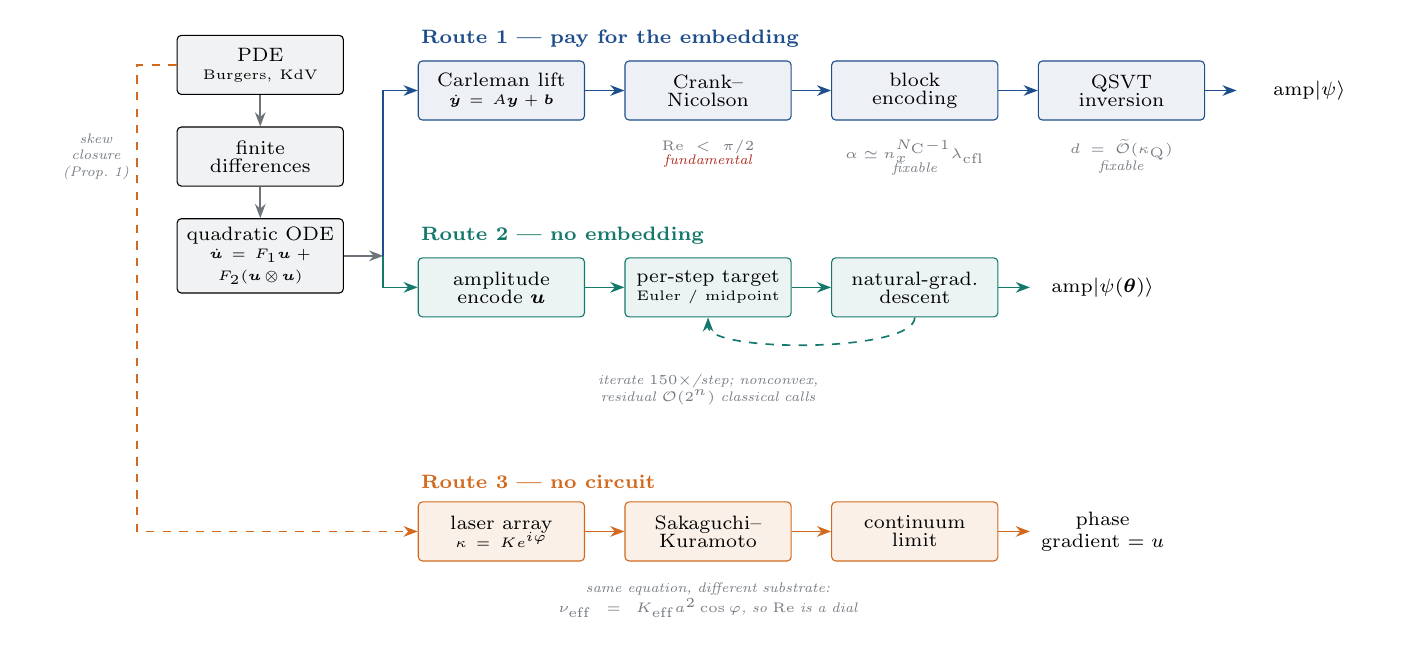
\begin{tikzpicture}[
  >={Stealth[length=1.8mm]},
  box/.style={draw,rounded corners=1.5pt,align=center,inner sep=3pt,
              minimum height=7.5mm,text width=19mm,font=\scriptsize,fill=palClassical!12},
  r1/.style={box,draw=palBlue,fill=palBlue!8},
  r2/.style={box,draw=palTeal,fill=palTeal!8},
  r3/.style={box,draw=palOrange,fill=palOrange!10},
  res/.style={align=center,font=\scriptsize,text width=16mm},
  cost/.style={font=\tiny\itshape,align=center,text=palClassical!85!black},
  tag/.style={font=\scriptsize\bfseries,align=left,inner sep=1pt},
  a/.style={->,semithick,palClassical!80!black},
  ab/.style={->,semithick,palBlue},
  arrt/.style={->,semithick,palTeal},
  ao/.style={->,semithick,palOrange},
  node distance=5mm,
]

% ================= shared trunk (vertical, far left) =================
\node[box] (pde) at (0,0) {PDE\\[-1.5pt]\tiny Burgers, KdV};
\node[box,below=4mm of pde] (disc) {finite\\[-1.5pt]differences};
\node[box,below=4mm of disc] (ode) {quadratic ODE\\[-1.5pt]
   \tiny$\dot{\bm u}=F_1\bm u+F_2(\bm u\!\otimes\!\bm u)$};
\draw[a] (pde) -- (disc);
\draw[a] (disc) -- (ode);
\node[cost,left=1.5mm of disc,text width=15mm] {skew\\ closure\\ (Prop.~1)};

\coordinate (br) at ($(ode.east)+(5mm,0)$);
\draw[a] (ode) -- (br);

% ================= Route 1 : top lane =================
\node[r1] (carl) at ($(br)+(15mm,21mm)$) {Carleman lift\\[-1.5pt]
   \tiny$\dot{\bm y}=A\bm y+\bm b$};
\node[r1,right=5mm of carl] (cn)   {Crank--\\[-1.5pt]Nicolson};
\node[r1,right=5mm of cn]   (be)   {block\\[-1.5pt]encoding};
\node[r1,right=5mm of be]   (qsvt) {QSVT\\[-1.5pt]inversion};
\node[res,right=4mm of qsvt] (st1) {$\mathrm{amp}\ket{\psi}$};

\draw[ab] (br) |- (carl);
\draw[ab] (carl) -- (cn);
\draw[ab] (cn) -- (be);
\draw[ab] (be) -- (qsvt);
\draw[ab] (qsvt) -- (st1);

\node[tag,text=palBlue,above=1.2mm of carl.north west,anchor=south west]
  {Route 1 \textemdash\ pay for the embedding};
\node[cost,below=1.2mm of cn,text width=21mm]
  {$\Rey<\pi/2$\\[-1pt]\textcolor{palRed}{fundamental}};
\node[cost,below=1.2mm of be,text width=22mm]
  {$\alpha\!\simeq\!n_x^{\NC-1}\lambda_{\rm cfl}$\\[-1pt]fixable};
\node[cost,below=1.2mm of qsvt,text width=20mm]
  {$d=\Ot(\kQ)$\\[-1pt]fixable};

% ================= Route 2 : middle lane =================
\node[r2] (amp) at ($(br)+(15mm,-4mm)$) {amplitude\\[-1.5pt]encode $\bm u$};
\node[r2,right=5mm of amp] (targ) {per-step target\\[-1.5pt]\tiny Euler / midpoint};
\node[r2,right=5mm of targ] (ngd) {natural-grad.\\[-1.5pt]descent};
\node[res,right=4mm of ngd] (st2) {$\mathrm{amp}\ket{\psi(\bm\theta)}$};

\draw[arrt] (br) |- (amp);
\draw[arrt] (amp) -- (targ);
\draw[arrt] (targ) -- (ngd);
\draw[arrt] (ngd) -- (st2);
\draw[arrt,dashed] (ngd.south) .. controls +(0,-4.5mm) and +(0,-4.5mm) .. (targ.south);

\node[tag,text=palTeal,above=1.2mm of amp.north west,anchor=south west]
  {Route 2 \textemdash\ no embedding};
\node[cost,below=6mm of targ,text width=30mm]
  {iterate $150\times$/step; nonconvex, residual $\Oh(2^n)$ classical calls};

% ================= Route 3 : bottom lane =================
\node[r3] (laser) at ($(br)+(15mm,-35mm)$) {laser array\\[-1.5pt]\tiny$\kappa=Ke^{i\varphi}$};
\node[r3,right=5mm of laser] (sk)  {Sakaguchi--\\[-1.5pt]Kuramoto};
\node[r3,right=5mm of sk]  (cont)  {continuum\\[-1.5pt]limit};
\node[res,right=4mm of cont] (st3) {phase gradient $=u$};

\draw[ao] (laser) -- (sk);
\draw[ao] (sk) -- (cont);
\draw[ao] (cont) -- (st3);
\draw[ao,dashed] (pde.west) -- ++(-5mm,0) |- (laser.west);

\node[tag,text=palOrange,above=1.2mm of laser.north west,anchor=south west]
  {Route 3 \textemdash\ no circuit};
\node[cost,below=1.5mm of sk,text width=52mm]
  {same equation, different substrate:
   $\nu_{\rm eff}=K_{\rm eff}a^2\cos\varphi$, so $\Rey$ is a dial};

\end{tikzpicture}
\caption{The three routes as one pipeline. All share the discretization and the exactly
energy-conserving convective closure (Proposition~\ref{prop:closure}), then diverge at the point where
each decides how to reconcile a nonlinear equation with linear hardware. Route~1 (blue) completes the
linear-embedding chain and pays for it at every stage; annotations mark where the cost accrues and
whether it is fixable, with the Carleman convergence threshold $\Rey<\pi/2$ the one obstruction that
is not. Route~2 (teal) stops at the amplitude encoding and moves the nonlinearity into a classical
optimizer, trading circuit depth for a nonconvex problem solved afresh each step. Route~3 (orange)
never digitizes: a coupled laser array whose continuum limit \emph{is} Burgers, in which the Reynolds
number that obstructs Route~1 becomes a tunable coupling phase.}
\label{fig:pipeline}
\end{figure*}

\noindent
Three contributions distinguish this work from a survey of the alternatives.

First, all three routes are held to the same physical standard. We prove
(Sec.~\ref{sec:closure}) that the skew-symmetric convective closure is what makes the required $L^2$
bounds hold \emph{exactly and at any resolution}, and we prove (Sec.~\ref{sec:euler}) that forward
Euler injects energy into KdV's conservative ODE on every step regardless of stepsize, whereas
implicit midpoint conserves it exactly. These are not incidental numerical hygiene: without the first,
a discretization violates the very bound that defines the target physics, and without the second, a
variational propagator inherits a systematic drift that no amount of circuit fidelity can remove.

Second, we separate \emph{measured} from \emph{projected} performance throughout, and label every
number accordingly. Sections~\ref{sec:carleman} and~\ref{sec:variational} report circuits we built,
transpiled, and ran; Sec.~\ref{sec:cost} reports asymptotics we derived and calibrated against
published gate-level data~\cite{Setty2026}. Conflating the two is, in our reading, the main way
resource estimates for this problem class become misleading.

Third, we localize the obstruction. Of the five cost drivers in Route~1, the qubit count is a clean
exponential win that nothing erodes; the block encoding and the sequential time-stepping are large but
fixable; the readout is a hard information-theoretic barrier only if the full field is wanted; and
exactly one --- the Carleman convergence radius --- is fundamental within the framework. That
decomposition, rather than a single headline number, is what we regard as the useful output.

Figure~\ref{fig:pipeline} shows the three routes as one pipeline, with the stage at which each
declines to continue down the linear-embedding chain, and where each one's cost accumulates.
Table~\ref{tab:notation} fixes notation across the three routes, which are drawn from formulations
that use conflicting symbols in the literature.

\begin{table}[t]
\caption{Notation used throughout. Where the underlying literature conflicts, we adopt the
convention in the right-hand column.}
\label{tab:notation}
\begin{ruledtabular}
\begin{tabular}{ll}
Symbol & Meaning \\
\hline
$n_x$ & number of spatial grid points \\
$n$ & qubits in the field register, $n_x=2^n$ \\
$\NC$ & Carleman truncation order \\
$\Rey=UL/\nu$ & Reynolds number ($U=\norm{u_0}_\infty$, $L=1$) \\
$\Rey_\Delta$ & cell Reynolds number, $U\Delta x/\nu$ \\
$\epsilon$ & target relative error \\
$\alpha$ & block-encoding subnormalization \\
$\kQ$ & effective condition number, $\alpha/\sigma_{\min}$ \\
$\kappa_V$ & eigenvector condition number of $A$ \\
$P$ & variational ansatz parameter count \\
$m$ & number of timesteps \\
\end{tabular}
\end{ruledtabular}
\end{table}

%=======================================================================
\section{The shared physical problem}
\label{sec:discretization}
%=======================================================================

All three routes describe the same physics, and Routes~1 and~2 share one discretization. We set it up
here, and prove the two structural facts that everything downstream depends on.

\subsection{Discretization}

Both PDEs are discretized on $n_x$ periodic grid points $x_i=i/n_x$, spacing $\Delta x=1/n_x$, with
central finite differences~\cite{Fornberg1988}. Writing $u_i\approx u(x_i,t)$, the first, second, and
third derivatives are the circulant matrices
\begin{align}
(D_1)_{i,i\pm1}&=\pm\tfrac{1}{2\Delta x},\\
(D_2)_{i,i\pm1}&=\tfrac{1}{\Delta x^2},\quad (D_2)_{ii}=-\tfrac{2}{\Delta x^2},\\
(D_3)_{i,i\pm1}&=\mp\tfrac{1}{\Delta x^3},\quad (D_3)_{i,i\pm2}=\pm\tfrac{1}{2\Delta x^3},
\end{align}
all with periodic wraparound. Both equations then take the quadratic form
\begin{equation}
\dot{\bm u} = F_1\bm u + F_2(\bm u\otimes\bm u),
\label{eq:quadratic-ode}
\end{equation}
with $F_1=\nu D_2$ for Burgers, $F_1=-\delta D_3$ for KdV, and $F_2$ a fixed bilinear operator
representing $-u\,\partial_xu$ acting on the length-$n_x^2$ vector $\bm u\otimes\bm u$.

\subsection{The convective closure must be chosen with care}
\label{sec:closure}

The naive central-difference convective term,
$(F_2^{\rm naive}(\bm u\otimes\bm u))_i=-\tfrac{1}{2\Delta x}u_i(u_{i+1}-u_{i-1})$, does \emph{not}
satisfy $\bm u^{\!\top}F_2^{\rm naive}(\bm u\otimes\bm u)=0$ for generic $\bm u$ --- only for specially
symmetric inputs, by coincidence. Since
$\tfrac{d}{dt}\norm{\bm u}_2^2=2\bm u^{\!\top}F_1\bm u+2\bm u^{\!\top}F_2(\bm u\otimes\bm u)$ and
$\bm u^{\!\top}F_1\bm u\le0$ for Burgers' dissipative $F_1$, the sign of the derivative is guaranteed
only if the second term vanishes identically; otherwise nothing prevents the discrete norm from
growing, in direct violation of the maximum principle. We therefore use the skew-symmetric
(energy-conserving) closure
\begin{equation}
F_2(\bm u\otimes\bm u)_i = -\tfrac{1}{3}\Big[u_i\,(D_1\bm u)_i+\big(D_1(\bm u\!\odot\!\bm u)\big)_i\Big],
\label{eq:f2skew}
\end{equation}
with $\odot$ the elementwise product --- half the naive form plus half its conservative flux
counterpart, the standard structure of energy-conserving treatments of nonlinear
advection~\cite{Harten1983,Tadmor1987}.

\begin{proposition}
\label{prop:closure}
$\bm u^{\!\top}F_2(\bm u\otimes\bm u)=0$ identically, for every $\bm u\in\R^{n_x}$.
\end{proposition}
\begin{proof}
$D_1$ is antisymmetric: $(D_1)_{i,i+1}=\tfrac{1}{2\Delta x}=-(D_1)_{i+1,i}$, so $D_1^{\!\top}=-D_1$
and $\bm a^{\!\top}D_1\bm b=-\bm b^{\!\top}D_1\bm a$ for any $\bm a,\bm b$. Applying this with
$\bm a=\bm u$, $\bm b=\bm u\odot\bm u$ gives
$\bm u^{\!\top}D_1(\bm u\odot\bm u)=-(\bm u\odot\bm u)^{\!\top}D_1\bm u=-\sum_iu_i^2(D_1\bm u)_i$,
while the first bracket contracted with $\bm u$ is term by term $\sum_iu_i^2(D_1\bm u)_i$. The two
cancel.
\end{proof}

We verified this to machine precision ($\sim10^{-17}$) with random vectors at every size used here,
and separately verified that Eq.~\eqref{eq:f2skew} agrees with $-u\,\partial_xu$ to the expected
$\Oh(\Delta x^2)$ truncation order. The naive form fails the exact-zero test for generic $\bm u$ by an
$\Oh(1)$ amount that grows with $n_x$: in a KdV run it produced an $11\%$ drift in $\norm{u(t)}_2$
over the simulated interval, for an equation that conserves it exactly.

With the closure of Eq.~\eqref{eq:f2skew}, $\tfrac{d}{dt}\norm{\bm u}_2^2=2\bm u^{\!\top}F_1\bm u$ for
\emph{both} PDEs at \emph{any} resolution. For Burgers this is $\le0$, so $\norm{u(t)}_2$ is
non-increasing; for KdV, $F_1=-\delta D_3$ is itself antisymmetric by the same argument, so it
vanishes and $\norm{u(t)}_2$ is exactly conserved.

\subsection{Exact conservation of the ODE does not survive time discretization}
\label{sec:euler}

Proposition~\ref{prop:closure} concerns the exact flow of Eq.~\eqref{eq:quadratic-ode} and says
nothing about a time-stepping scheme. Take one forward-Euler step
$\bm u_{n+1}=\bm u_n+\Delta t\,f(\bm u_n)$ with $f(\bm u)=F_1\bm u+F_2(\bm u\otimes\bm u)$ the KdV
right-hand side, for which $\bm u^{\!\top}f(\bm u)=0$ exactly. Then
\begin{align}
\norm{\bm u_{n+1}}_2^2
&=\norm{\bm u_n}_2^2+2\Delta t\,\bm u_n^{\!\top}f(\bm u_n)+\Delta t^2\norm{f(\bm u_n)}_2^2\notag\\
&=\norm{\bm u_n}_2^2+\Delta t^2\norm{f(\bm u_n)}_2^2\;\ge\;\norm{\bm u_n}_2^2 .
\label{eq:euler-injects}
\end{align}
Forward Euler therefore \emph{provably} injects energy into KdV's exactly conservative ODE on every
step, however small $\Delta t$ is. We confirmed Eq.~\eqref{eq:euler-injects} numerically to $10^{-16}$
relative precision. The remedy, with its own exactness proof, is the implicit midpoint rule
(Sec.~\ref{sec:midpoint}); the observed consequence of ignoring it is a monotone growth
$\norm{\bm u}_2 = 1.00\to1.19\to1.42\to1.72$ over three steps.

\subsection{The Reynolds number sets the resolution both digital routes need}
\label{sec:reynolds}

Non-dimensionalizing Eq.~\eqref{eq:burgers} by amplitude $U=\norm{u_0}_\infty$ and domain length
$L=1$ leaves the single parameter $\Rey=UL/\nu$. Proposition~\ref{prop:closure} guarantees an energy
bound but not monotonicity; central differences on the convective term are monotonicity-preserving
only if the cell Reynolds number satisfies $\Rey_\Delta=U\Delta x/\nu\lesssim2$. We confirmed this
bound two independent ways: by linearizing the discrete update near $u\approx U$ and requiring the
off-diagonal coefficients to stay non-negative, and by the spectral analysis of
Sec.~\ref{sec:cost}. Table~\ref{tab:reynolds} evaluates both numbers for the systems used here.

\begin{table}[t]
\caption{Reynolds and cell Reynolds numbers for the Burgers systems solved in this work ($L=1$).
The variational grid sits a factor of six above the monotonicity threshold, a coarse-grid overshoot
we report rather than conceal; $\Rey_\Delta\le2$ at $\nu=0.01$ requires $n_x\gtrsim50$.}
\label{tab:reynolds}
\begin{ruledtabular}
\begin{tabular}{lccc}
System & $\nu$ & $\Rey$ & $\Rey_\Delta$ \\
\hline
Route 1, Carleman ($n_x=5$) & 0.1 & 9.5 & 1.9 \\
Route 2, variational ($n_x=8$) & 0.01 & 100 & 12.5 \\
Threshold $\Rey_\Delta\le2$ requires & 0.01 & 100 & $n_x\gtrsim50$ \\
\end{tabular}
\end{ruledtabular}
\end{table}

%=======================================================================
\section{Route 1: Carleman--QSVT, as built}
\label{sec:carleman}
%=======================================================================

This section reports what we constructed and measured. Its asymptotic cost is deferred to
Sec.~\ref{sec:cost} so that measured and projected quantities are never mixed.

\subsection{The Carleman lift}

Carleman linearization introduces the tensor hierarchy
$\bm y=(\bm u,\ \bm u^{\otimes2},\ \dots,\ \bm u^{\otimes\NC})^{\!\top}$, on which
Eq.~\eqref{eq:quadratic-ode} becomes the \emph{linear} system
\begin{equation}
\dot{\bm y}=A\bm y+\bm b,
\label{eq:carleman}
\end{equation}
with $A$ block upper-bidiagonal: the diagonal block $A_{jj}$ propagates $\bm u^{\otimes j}$ under
$F_1$ and the superdiagonal block $A_{j,j+1}$ couples it to $\bm u^{\otimes(j+1)}$ through $F_2$.
Truncating at order $\NC$ (setting $\bm u^{\otimes(\NC+1)}\equiv0$) closes the system at dimension
$\sum_{j=1}^{\NC}n_x^j$.

The convergence theorem for this truncation~\cite{Liu2021} requires $F_1$ to be strictly dissipative
and controls the error through the ratio
$R=\norm{\bm u_0}_2\norm{F_2}_2/|\mathrm{Re}\,\mu_1(F_1)|$, with $\mu_1$ the eigenvalue of largest
real part. For our \emph{periodic} construction this theorem does not literally apply: the periodic
Laplacian has a zero (DC) mode, so $\mathrm{Re}\,\mu_1(F_1)=0$ exactly and $R$ diverges. The same is
true a fortiori for KdV, where $F_1$ is skew-symmetric. We therefore validated the truncation order
empirically instead, and report it as such: $\NC=2$ and $\NC=3$ give near-identical RMSE against a
high-accuracy RK45 reference, so at these parameters the truncation is not what limits accuracy; the
dispersion stiffness $\delta/\Delta x^3$ at fixed $\Delta t$ is, which is why $\delta$ is kept small.
Section~\ref{sec:carleman-conv} returns to what the convergence condition costs when it \emph{is}
enforced.

\subsection{Time marching and block encoding}

Each timestep is a linear solve. We use Crank--Nicolson (trapezoidal) marching,
\begin{equation}
\Big(I-\tfrac{\Delta t}{2}A\Big)\bm y_{n+1}=\Big(I+\tfrac{\Delta t}{2}A\Big)\bm y_n,
\label{eq:cn}
\end{equation}
rather than implicit Euler: the block-encoded matrix is the same, but the local error is
$\Oh(\Delta t^2)$ instead of $\Oh(\Delta t)$, which we checked classically to need roughly $20\times$
fewer timesteps at matched accuracy, following the higher-order rescaling analysis of
Ref.~\cite{Costa2025}.

We implemented and compared two block encodings of the Crank--Nicolson matrix: a dense
arbitrary-unitary construction, and one built from the matrix's Pauli decomposition as a linear
combination of unitaries (LCU). The comparison produced a result worth stating explicitly, because
it inverts the usual intuition. The Pauli-LCU encoding is the \emph{more} expensive of the two for
this matrix family, by two to three orders of magnitude, because the Kronecker-shift structure of
Eq.~\eqref{eq:carleman} is sparse in the computational basis but \emph{dense} in the Pauli basis.
Sparsity in one basis buys nothing if the encoding reads the other.

\subsection{QSVT inversion, and what we verified}

Matrix inversion is performed by QSVT~\cite{Gilyen2019} applied to the block encoding, with phase
angles generated for a target condition number $\kappa=8$ ($561$ angles). Table~\ref{tab:carleman}
lists the systems solved and Table~\ref{tab:carleman-resources} their exact transpiled cost.

Every quantum result agrees with its classical linear-algebra counterpart to numerical precision.
Both notebooks compare three solvers --- the exact untruncated nonlinear ODE integrated by RK45, the
Carleman-truncated system solved exactly (isolating truncation error), and the Carleman-truncated
system solved by QSVT under both encodings --- so a disagreement would localize to a specific stage.
None appeared.

The gate counts in Table~\ref{tab:carleman-resources} should be read as a property of the
\emph{encoding we chose}, not of Carleman--QSVT as such, and the distinction is worth stating
plainly. Our dense construction assembles the full $2^{n_w}\times2^{n_w}$ dilation
$\big[\begin{smallmatrix} A_s & \sqrt{I-A_sA_s^\dagger}\\ \sqrt{I-A_s^\dagger A_s} &
-A_s^\dagger\end{smallmatrix}\big]$ explicitly and hands it to the transpiler as an opaque unitary.
By that point the Carleman matrix's sparsity and Kronecker-shift structure have been destroyed: the
transpiler sees an arbitrary unitary and falls back on generic
synthesis~\cite{Shende2006}, which is precisely the $\Oh(4^{n_w})$ cost we measure in
Sec.~\ref{sec:blockenc}. The QSVT projector layers, by contrast, are built as multi-controlled phase
gates rather than dense diagonal matrices, so the blow-up is localized to the block-encoding layers
alone. What a structure-aware encoding would cost instead is the subject of
Sec.~\ref{sec:blockenc}, and is the reason the subnormalization analysis there matters. Figure~\ref{fig:carleman-burgers} shows the resulting Burgers propagation,
Fig.~\ref{fig:carleman-time} the per-timestep RMSE, post-selection success probability, and
amplitude-encoding fidelity, and Fig.~\ref{fig:carpet} the classical space--time reference.

\begin{table}[t]
\caption{Route~1 systems solved ($\NC=2$, $\Delta t=0.1$, $t\in[0,0.3]$). $\kQ$ is the measured
effective condition number of the encoded matrix, which sets the required QSVT degree.}
\label{tab:carleman}
\begin{ruledtabular}
\begin{tabular}{lcccc}
PDE & $n_x$ & $\dim A$ & $\kQ$ (dense) & $\kQ$ (LCU) \\
\hline
Burgers ($\nu=0.1$) & 5 & 30 & 9.35 & 8.79 \\
KdV ($\delta=0.0625$) & 4 & 20 & 4.02 & 4.75 \\
\end{tabular}
\end{ruledtabular}
\end{table}

\begin{table}[t]
\caption{\textbf{Measured.} Exact transpiled cost of one QSVT matrix inversion, $\kappa=8$ ($561$
phase angles), $\{\mathrm{cx},u_3\}$ basis. This is paid at \emph{every} timestep.}
\label{tab:carleman-resources}
\begin{ruledtabular}
\begin{tabular}{llrrr}
PDE & encoding & qubits & gates & CX gates \\
\hline
Burgers & dense & 6 & 2{,}612{,}767 & 996{,}697 \\
Burgers & Pauli-LCU & 14 & 1{,}716{,}882{,}557 & 803{,}286{,}678 \\
KdV & dense & 6 & 2{,}610{,}531 & 996{,}697 \\
KdV & Pauli-LCU & 13 & 396{,}632{,}217 & 185{,}505{,}488 \\
\end{tabular}
\end{ruledtabular}
\end{table}

\begin{figure*}[t]
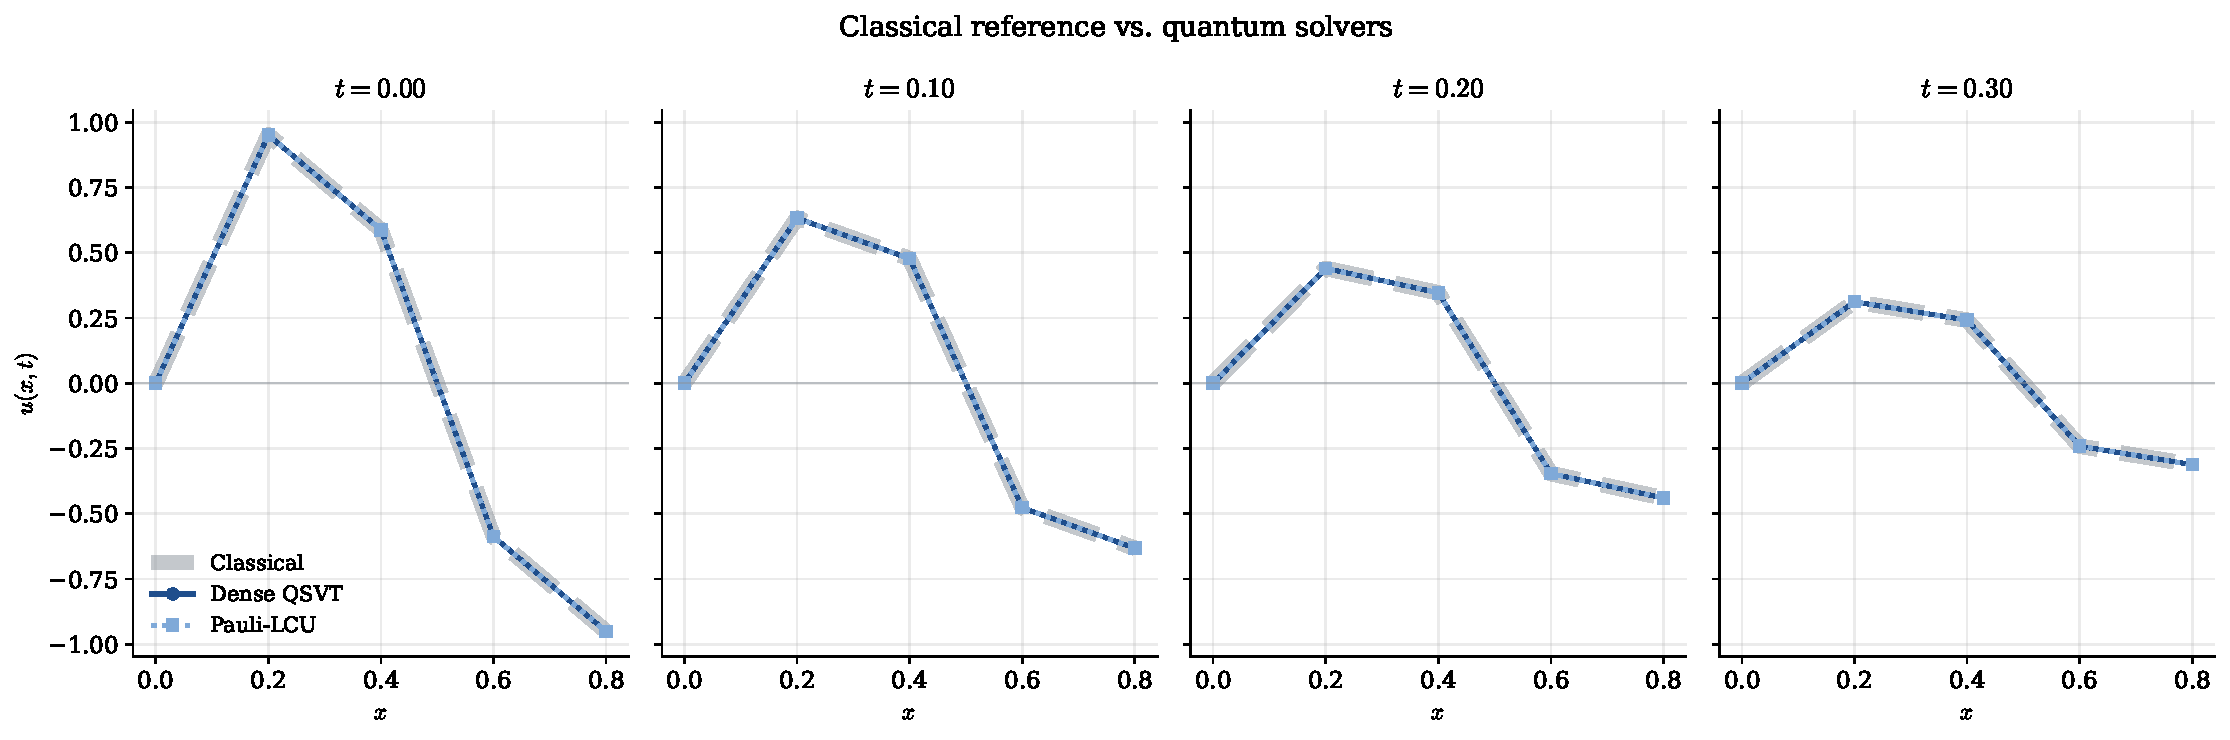
\includegraphics[width=\textwidth]{figures/fig_burgers_carleman.pdf}
\caption{Burgers propagation via Route~1: classical (dashed) versus dense QSVT (solid) versus
Pauli-LCU QSVT (dotted). At $\nu=0.1$ diffusion dominates advection, so the profile decays and mildly
skews rather than steepening into a shock. The three curves coincide to numerical precision, which is
the point of the figure: both block encodings implement the same Carleman-lifted operator $A$
correctly, not merely a plausible one.}
\label{fig:carleman-burgers}
\end{figure*}

\begin{figure}[t]
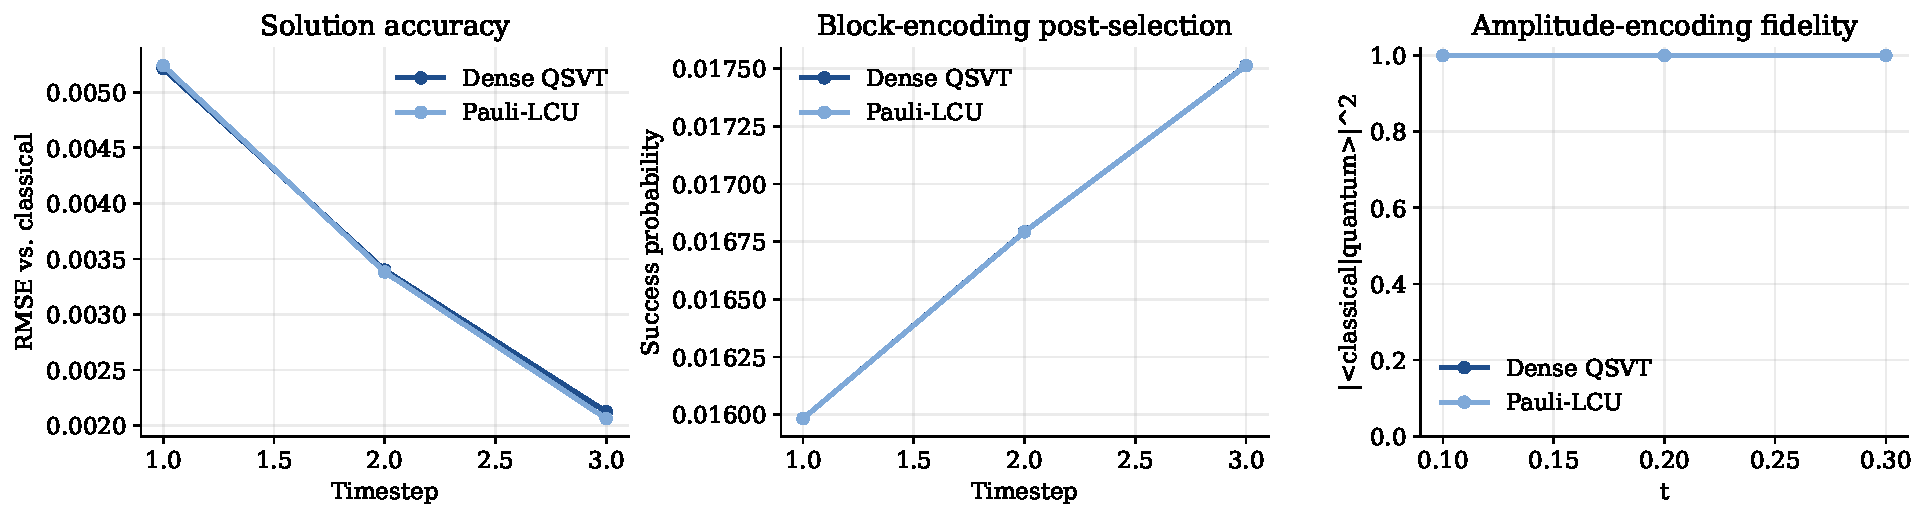
\includegraphics[width=\columnwidth]{figures/fig_burgers_timemarching.pdf}
\caption{Per-timestep RMSE against the classical reference, QSVT post-selection success probability,
and amplitude-encoding fidelity, for both block encodings. Success probability is the quantity that
compounds over a sequential run, and Sec.~\ref{sec:sequential} shows why that compounding is fatal
without a dilation.}
\label{fig:carleman-time}
\end{figure}

\begin{figure}[t]
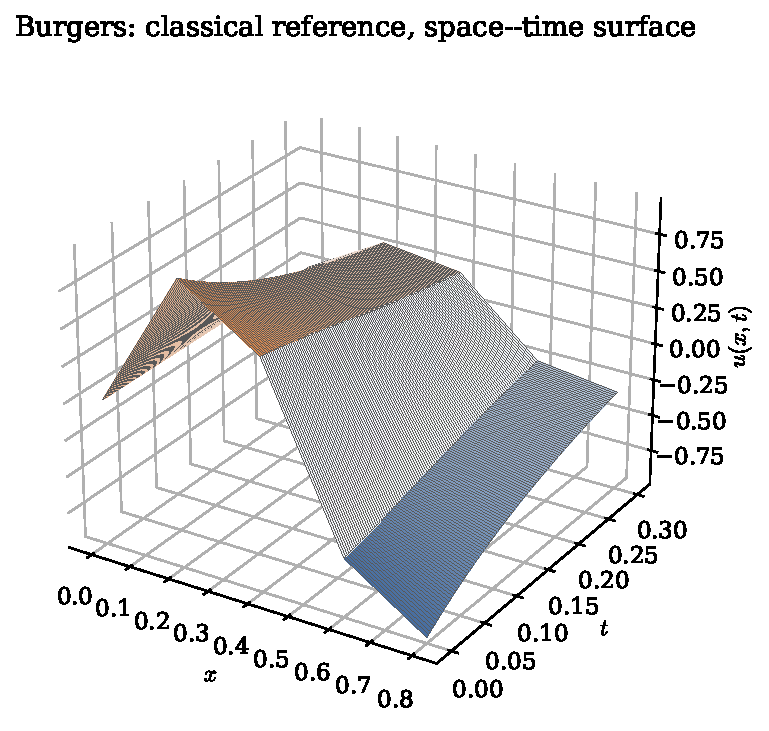
\includegraphics[width=\columnwidth]{figures/fig_burgers_carpet.pdf}
\caption{Classical space--time reference solution for the Burgers instance of
Table~\ref{tab:carleman} (finely sub-stepped, for visualization). Both digital routes are checked
against this surface at every timestep.}
\label{fig:carpet}
\end{figure}

%=======================================================================
\section{What Route 1 costs}
\label{sec:cost}
%=======================================================================

We now derive the asymptotic cost of the pathway. Every quantity in this section is
\emph{projected}, not measured; where possible the projections are calibrated against published
gate-level data for a $30\times30$ Burgers instance~\cite{Setty2026}, and we state the agreement.
Our reconstructed data-element count, subnormalization, effective condition number, and success
probability all reproduce the published values --- the success-probability model to $5\%$ and the
subnormalization formula exactly --- which is what licenses extrapolating them.

\subsection{The error budget, and which errors are amplified}

The pipeline accumulates five error sources: spatial discretization, Carleman truncation, time
discretization, QSVT polynomial approximation, and statistical (shot) error. They are not
interchangeable. Errors incurred \emph{before} the linear solve are amplified by the effective
condition number $\kQ$ when propagated through it, while errors incurred \emph{by} the solve are not.
This distinction determines the budget allocation and is why a seemingly modest input error can
dominate the final cost.

\subsection{The binding constraint: Carleman convergence requires $\Rey<\pi/2$}
\label{sec:carleman-conv}

This is the deepest limitation of the route, and it is a statement about the physics, not the
hardware. The standard analysis~\cite{Liu2021,Forets2017} of the quadratic system requires $F_1$
dissipative and controls the truncation error by
\begin{equation}
R:=\frac{\norm{\bm u_0}_2\,\norm{F_2}_2}{|\mathrm{Re}\,\mu_1(F_1)|},
\qquad
\NC=\left\lceil\frac{\ln(1/\epsilon)}{\ln(1/R)}\right\rceil ,
\label{eq:Rdef}
\end{equation}
valid only for $R<1$; if $R\ge1$ no such bound exists and increasing $\NC$ is not guaranteed to help.

Evaluated naively for the Dirichlet discretization, $R\simeq\Rey\,n_x^{3/2}/2\pi^2$ grows with grid
refinement --- which cannot be physical, since refining a grid does not make a PDE more nonlinear.
The inflation comes from using the unweighted operator norm of $F_2$, which measures its action on all
of $\R^{n_x^2}$, whereas the dynamics only ever visits the tensor manifold
$\{\bm u\otimes\bm u\}$. Restricting to that manifold,
$[F_2\bm u^{\otimes2}]_j\approx-u_j(\partial_xu)_j$, so
$\norm{F_2\bm u^{\otimes2}}/\norm{\bm u}\le\norm{\partial_xu}_\infty$, which is grid-independent.
With $\mu_1(F_1)\to-\pi^2\nu/L^2$ as $\Delta x\to0$ and $\norm{\partial_xu}_\infty=2\pi U/L$ for
$u_0=U\sin(2\pi x/L)$, the sharpened ratio is
\begin{align}
R_\star&=\frac{\norm{\partial_xu}_\infty}{\pi^2\nu/L^2}=\frac{2}{\pi}\Rey,\notag\\
&\Longrightarrow\quad R_\star<1\iff\Rey<\tfrac{\pi}{2}\approx1.57 .
\label{eq:Rstar}
\end{align}

The conclusion is robust to how it is computed: for a published $\Rey=100$ instance the naive
estimate gives $R=56.6$, the sharpened estimate $R_\star=63.7$, and direct evaluation of
Eq.~\eqref{eq:Rdef} from the assembled matrices gives $R=76.2$. All three place that instance two
orders of magnitude outside the provably convergent regime. Figure~\ref{fig:carleman-threshold}(a)
shows $\NC$ diverging as $\Rey\to\pi/2$.

\begin{remark}[Rescaling does not help]
Rescaling $\bm u\to\bm u/\Gamma$ to shrink $\norm{\bm u_0}$ leaves Eq.~\eqref{eq:quadratic-ode}
satisfied with $F_2\to\Gamma F_2$, so the product $\norm{\bm u_0}\norm{F_2}$ in Eq.~\eqref{eq:Rdef}
is unchanged. The constraint is physical, not a normalization artifact.
\end{remark}

\begin{remark}[KdV is worse, not better]
For KdV, $F_1$ is skew-symmetric and $\mathrm{Re}\,\mu_1=0$ exactly, so $R=\infty$ and
Eq.~\eqref{eq:Rdef} is vacuous. One must fall back on finite-horizon bounds of the form
$\varepsilon_{\rm CL}\lesssim\norm{\bm u_0}(T/\tau_{\rm nl})^{\NC}$ with
$\tau_{\rm nl}=\norm{\partial_xu}_\infty^{-1}$~\cite{Wu2025}, which converge only for $T$ less than
roughly one eddy turnover. Restarting is not an escape, because re-preparing an amplitude encoding of
$\bm u(T)$ requires tomography.
\end{remark}

\begin{figure*}[t]

\includegraphics[width=\textwidth]{figures/fig_carleman.pdf}
\caption{\textbf{Projected.} (a) Carleman order $\NC$ required by Eq.~\eqref{eq:Rdef} to reach
relative error $\epsilon$, using the sharpened ratio $R_\star=2\Rey/\pi$. Beyond $\Rey=\pi/2$ (red
line) the series has no proven convergence regime and no finite $\NC$ suffices --- this is the binding
constraint on the entire route. (b) The block-1 post-selection probability, which decays
geometrically in $\NC$ unless the state is rescaled so that $\gamma=\norm{\bm u}_2<1$.}
\label{fig:carleman-threshold}
\end{figure*}

\subsection{The block encoding, not the matrix, is the largest avoidable cost}
\label{sec:blockenc}

For the coherent-permutation block encoding, the subnormalization obeys
\begin{equation}
\alpha_{\rm cp}\simeq n_x^{\,\NC-1}\lambda_{\rm cfl},
\qquad \lambda_{\rm cfl}=\Delta t/\Delta x,
\label{eq:alphacp}
\end{equation}
which we confirmed numerically [Fig.~\ref{fig:alpha}]. Because $\alpha$ enters the cost linearly
through $\kQ=\alpha/\sigma_{\min}$, the algorithm is polynomial in grid size and \emph{exponential in
the Carleman order} --- precisely the scaling the Carleman embedding was supposed to avoid. Replacing
it with an arithmetic sparse-access oracle, which indexes the $\Oh(\NC)$ nonzero entries per row
directly rather than synthesizing a dense unitary, restores
\begin{equation}
\alpha_{\rm sp}=\Oh(\NC^2\lambda_{\rm diff}),
\label{eq:alphasp}
\end{equation}
independent of $n_x$ except through the diffusion number. The gap is already a factor of $17$ at
$n_x=15$, $\NC=3$. This is an engineering problem with a known fix, and we treat it as such below.

A complementary and independently measured statement holds for our own dense construction of
Sec.~\ref{sec:carleman}: its per-layer gate count fits $\propto2^{2.03n_w}=\Oh(4^{n_w})$ against its
own qubit count $n_w$, the generic cost of synthesizing an arbitrary unitary with no exploitable
structure~\cite{Shende2006}, giving $\Oh(n_x^4)$ in grid size at $\NC=2$. The two statements identify
the same lesson from opposite directions, one asymptotic and one measured: the encoding, not the
matrix, dominates. A structure-blind encoding pays $\Oh(4^{n_w})$ in synthesis; a structure-aware but
subnormalization-blind one pays $n_x^{\NC-1}$ in QSVT degree. Neither cost is intrinsic to the
Carleman lift, which is why we regard both as engineering problems rather than obstructions ---
in sharp contrast to the convergence threshold of Sec.~\ref{sec:carleman-conv}, which is neither.

\begin{figure*}[t]

\includegraphics[width=\textwidth]{figures/fig_alpha.pdf}
\caption{Growth of the block-encoding subnormalization $\alpha$, which sets the effective condition
number and hence the QSVT degree. (a) Versus grid size at $\NC=2$: the coherent-permutation encoding
(cp) tracks $\propto n_x^2$ while the sparse arithmetic oracle (sp) grows far more slowly. (b) Versus
Carleman order: cp grows geometrically in $\NC$, sp does not.
Equations~\eqref{eq:alphacp}--\eqref{eq:alphasp} are the corresponding closed forms. Neither encoding
is constructed as a circuit here: $\alpha$ is evaluated exactly from the assembled Carleman matrix
($\alpha_{\rm cp}$ as the sum of $|{\cdot}|$ over distinct value/diagonal-offset pairs,
$\alpha_{\rm sp}=s\norm{L}_{\max}$), so these are exact cost-model constants rather than measured
circuit resources. The circuits we did build are the dense and Pauli-LCU encodings of
Table~\ref{tab:carleman-resources}.}
\label{fig:alpha}
\end{figure*}

\subsection{Sequential time stepping does not scale, and the fix has a bonus}
\label{sec:sequential}

Solving one implicit step at a time --- the natural reading of Eq.~\eqref{eq:cn}, and what our own
implementation does --- is not viable asymptotically. Each solve is heralded with probability
$p_s<1$, and the output of one step is the input of the next, so chaining $m$ steps costs
$\Oh(p_s^{-m/2})$ even with optimal amplitude amplification. This is the practical meaning of the
success-probability panel in Fig.~\ref{fig:carleman-time}.

The remedy is the dilated ``history-state'' formulation, which solves for all timesteps at once in a
single enlarged linear system. It comes with a genuinely useful surprise: the product $\alpha m$
entering the dilated system's condition number is \emph{independent of $\Delta t$}. Refining the time
step multiplies the number of steps and divides the subnormalization by the same factor, so nothing is
lost. This cancellation is what makes the assembled estimate below finite at all.

\subsection{Assembled scaling}
\label{sec:assembled}

Combining the above under stated assumptions --- sparse-oracle block encoding, high-order time
integration, history-state dilation, normalized initial data, $\Rey<\pi/2$ so that $\NC$ is finite,
and a grid that resolves the solution --- the sequential two-qubit depth is
\begin{equation}
\boxed{\;D_{\rm QSVT}=\Ot\!\left(\frac{\kappa_V\,T\,\NC^{3}}{\Rey\,\epsilon}\right),\;}
\label{eq:finaldepth}
\end{equation}
with
\begin{equation}
\NC=\Theta\!\left(\frac{\log(1/\epsilon)}{\log(\pi/2\Rey)}\right),\quad
\#\text{qubits}=\Theta\!\left(\frac{\log^2(1/\epsilon)}{\log(\pi/2\Rey)}\right).
\end{equation}
The depth model underlying Eq.~\eqref{eq:finaldepth} is calibrated against published gate-level depths
for four independent instances in Fig.~\ref{fig:depth}, and reproduces them within a factor of two.
Table~\ref{tab:assembled} collects the full breakdown.

\begin{figure}[t]

\includegraphics[width=0.85\columnwidth]{figures/fig_depth.pdf}
\caption{Calibration of the depth model against published two-qubit depths for four independent
circuit instances~\cite{Setty2026}. Dotted lines mark a factor of two. The agreement is what licenses
extrapolating the model to the regimes of Table~\ref{tab:worked}.}
\label{fig:depth}
\end{figure}

\begin{table}[t]
\caption{\textbf{Projected.} Assembled resource scaling for Route~1 under the assumptions of
Sec.~\ref{sec:assembled}. $\kappa_V$, the eigenvector condition number of the Carleman matrix, is the
least controlled quantity here: $A$ is strongly non-normal, and we are not aware of a bound on
$\kappa_V$ in the literature.}
\label{tab:assembled}
\begin{ruledtabular}
\begin{tabular}{lp{3.6cm}}
Resource & Scaling \\
\hline
Logical qubits & $\Theta(\NC\log n_x+\log m)$ \\
Carleman order $\NC$ & $\Theta(\log(1/\epsilon)/\log\tfrac{\pi}{2\Rey})$ \\
Grid points $n_x$ & $\Theta(\max(\Rey,\epsilon^{-1/2}))$ \\
Effective $\kQ$ & $\Oh(\kappa_V\NC T/(\Rey\,\epsilon))$ \\
Polynomial degree $d$ & $\Ot(\kQ)$ \\
\textbf{Total depth} & $\Ot(\kappa_V T\NC^{3}\Rey^{-1}\epsilon^{-1})$ \\
Shots, observable & $\Oh(\epsilon_{\rm obs}^{-1})$ \\
Shots, full field & $\Oh(n_x\epsilon^{-2})$ \\
\end{tabular}
\end{ruledtabular}
\end{table}

\subsection{A worked instance, against a laptop}

Table~\ref{tab:worked} evaluates Eq.~\eqref{eq:finaldepth} at the largest Reynolds number for which
the Carleman series provably converges, and places it beside a classical pseudo-spectral solve of the
same instance.

\begin{table}[t]
\caption{\textbf{Projected.} A worked instance at $\Rey=1$ (so $R_\star=0.637$), $\epsilon=10^{-3}$,
$T=0.3$, $n_x=128$. Depths are logical two-qubit gates; the required gate infidelity implies full
fault tolerance, with a further $10^3$--$10^4$ physical-qubit overhead per logical qubit.}
\label{tab:worked}
\begin{ruledtabular}
\begin{tabular}{lr}
Quantity & Value \\
\hline
Carleman order $\NC$ & 16 \\
System dimension & $2^{112}$ \\
Timesteps $m$ & 4915 \\
Subnormalization $\alpha_{\rm sp}$ & $2.0\times10^{3}$ \\
Dilated condition number & $1.0\times10^{7}$ \\
Polynomial degree $d$ & $2.3\times10^{8}$ \\
\textbf{Total depth} & $\bm{1.3\times10^{12}}$ \\
Total logical qubits & $\sim135$ \\
Required gate infidelity & $10^{-12}$ \\
Runtime at 100\,ns/gate & $\sim36$\,hours \\
\hline
\multicolumn{2}{l}{\emph{Classical pseudo-spectral, same instance}}\\
Arithmetic operations & $4.4\times10^{6}$ \\
Memory & 1\,kB \\
Runtime & $\sim1$\,ms \\
\end{tabular}
\end{ruledtabular}
\end{table}

The gap is roughly $10^6$ in operation count before error correction and $10^9$--$10^{10}$ after. Both
sides scale as $\Ot(\epsilon^{-1})$ in accuracy; the quantum side carries additional factors
$\kappa_V\NC^3$, its depth is inherently sequential where classical FFTs parallelize trivially, and it
returns a quantum state rather than a field.

One structural quantum win survives intact: the qubit count $\Oh(\NC d_{\rm sp}\log n_x)$ in $d_{\rm
sp}$ spatial dimensions is genuinely exponentially smaller than the classical $\Oh(n_x^{d_{\rm sp}})$,
and nothing in the analysis erodes it. Comparing work rather than memory, a crossover requires
$d_{\rm sp}\ge3$ before constants, and is conditional on all of $\Rey=\Oh(1)$, observable-only readout,
and $\kappa_V$ polynomially bounded.

\subsection{Why Burgers alone cannot settle the question}
\label{sec:colehopf}

There is an uncomfortable point specific to Burgers. The Cole--Hopf transformation
$u=-2\nu\,\partial_x\ln\phi$ maps Eq.~\eqref{eq:burgers} \emph{exactly} onto the linear heat equation
$\partial_t\phi=\nu\partial_{xx}\phi$. Burgers is therefore not a genuinely nonlinear test problem at
all: it is a linear problem in disguise, solvable classically in $\Oh(n_x\log n_x)$ total --- one FFT, a
diagonal multiplication, one inverse FFT --- for \emph{any} $T$ and \emph{any} $\Rey$, with no time
stepping whatsoever.

This does not invalidate Burgers as a benchmark for checking that circuits compile and produce the
right answer, which is how we use it. But it does mean a Burgers demonstration cannot by itself be
evidence that a method handles nonlinearity. The correct control is a PDE with no linearizing
substitution, which is exactly why we carry KdV through every stage of this work. We note in passing
that Cole--Hopf does not straightforwardly rescue the quantum route either: recovering $\ket{u}$ from
$\ket{\phi}$ requires the nonlinear map $\phi\mapsto\partial_x\ln\phi$ on amplitudes, which is not
implementable without tomography.

%=======================================================================
\section{Route 2: variational amplitude-encoded propagation}
\label{sec:variational}
%=======================================================================

Route~1 pays for linearity in circuit depth. Route~2 declines to pay: the nonlinearity is evaluated
by a classical optimizer, and the quantum register never holds anything larger than the field itself.
Everything in this section is measured.

\subsection{Encoding, ansatz, and cost function}

The field is represented as $\bm u=\mathrm{amp}\cdot\bm\psi(\bm\theta)$, with $\bm\psi(\bm\theta)$
the real, unit-norm statevector of an $n$-qubit \texttt{RealAmplitudes} ansatz ($n$ repetitions of
$R_y$ rotations with linear CNOT entanglement) and $\mathrm{amp}\in\R$ tracked classically. The ansatz
has exactly $P=n(n+1)$ parameters. Each timestep minimizes
\begin{align}
C(\bm\theta,\mathrm{amp}) &= \norm{\mathrm{amp}\cdot\bm\psi(\bm\theta)-\bm u_{\rm target}}_2^2,\\
\bm u_{\rm target}&=\bm u_{\rm old}+\Delta t\,f(\bm u_{\rm rhs}),
\label{eq:cost}
\end{align}
where $\bm u_{\rm rhs}=\bm u_{\rm old}$ for forward Euler (Burgers) or the implicit midpoint state
(KdV, Sec.~\ref{sec:midpoint}). Writing $C_0(\bm\theta)=\braket{\bm\psi(\bm\theta)}{\bm u_{\rm
target}}$ and minimizing over $\mathrm{amp}$ at fixed $\bm\theta$ gives $\mathrm{amp}^\star=C_0$; the
parameters then follow \emph{natural} gradient descent,
\begin{equation}
\bm\theta\leftarrow\bm\theta-\eta\,M(\bm\theta)^{+}\nabla_{\bm\theta}\big[-2\,\mathrm{amp}^\star C_0(\bm\theta)\big],
\label{eq:ngd}
\end{equation}
with $M^+$ the pseudo-inverse of the Fubini--Study metric and $\eta$ set by backtracking line search.
This is the standard cost-function form of the McLachlan principle~\cite{McLachlan1964,Yuan2019}.
What is specific to this work is that every ingredient of Eq.~\eqref{eq:ngd} is measured by a shallow
circuit with at most one ancilla and no controlled-ansatz operations anywhere.

\subsection{Circuit-level measurement}

Figure~\ref{fig:circuits} shows the four primitives. For a single-Pauli-rotation parameter the metric
diagonal is $M_{kk}=1/4$ exactly, needing no circuit; off-diagonal entries come from a single-ancilla
circuit inserting the two generators at the relevant gate positions and reading $\langle X\rangle$,
which we verified against a finite-difference evaluation of the exact Fubini--Study metric to
$\sim10^{-10}$. The overlaps entering $\bm u_{\rm target}$ --- identity, each shift term of $F_1$, and
the building blocks $\chi^\pm_i=(S^{\pm1}\bm\psi)_i\bm\psi_i$ and
$\mathrm{sq}^\pm_i=((S^{\pm1}\bm\psi)_i)^2$ required by the skew closure --- are each measured by a
compute--uncompute circuit whose all-zero outcome probability equals the squared overlap,
$P(0)=g^2$. The cyclic shift $S$ is implemented ancilla-free by a ripple-carry Toffoli chain.

\begin{figure}[t]
\centering
(a)\\
\begin{quantikz}[column sep=4pt,row sep=4pt]
& \gate{R_y(\theta_1)} & \ctrl{1} & \qw & \qw \\
& \gate{R_y(\theta_2)} & \targ{} & \ctrl{1} & \qw \\
& \gate{R_y(\theta_3)} & \qw & \targ{} & \qw
\end{quantikz}\\[6pt]
(b)\\
\begin{quantikz}[column sep=4pt,row sep=4pt]
\lstick{$q_0$} & \ctrl{2} & \ctrl{1} & \gate{X} & \qw \\
\lstick{$q_1$} & \ctrl{1} & \targ{} & \qw & \qw \\
\lstick{$q_2$} & \targ{} & \qw & \qw & \qw
\end{quantikz}\\[6pt]
(c)\\
\begin{quantikz}[column sep=3pt,row sep=4pt]
\lstick{anc:$\ket0$} & \gate{H} & \gate{X} & \ctrl{1} & \gate{X} & \qw & \ctrl{1} & \gate{H} & \meter{}\\
\lstick{sys} & \qw & \gate{U_{\rm bef}} & \gate{Y_k} & \qw & \gate{U_{\rm mid}} & \gate{Y_l} & \gate{U_{\rm aft}} & \qw
\end{quantikz}\\[6pt]
(d)\\
\begin{quantikz}[column sep=4pt,row sep=6pt]
\lstick{$A$} & \qwbundle{n} & \gate{U(\theta)} & \gate[2]{\text{CX}^{\otimes n}_{A\to B}} & \gate{U(\alpha)^\dagger} & \qw \\
\lstick{$B$} & \qwbundle{n} & \gate{U(\theta)\,S} & & \qw & \qw
\end{quantikz}
\caption{Circuit primitives of Route~2: (a) one repetition of the $R_y$/CNOT ansatz layer, applied $n$
times in total; (b) the ancilla-free cyclic shift $S$ (shown for $n=3$; the staircase of
$(n{-}1{-}k)$-controlled $X$ gates extends to any $n$); (c) the single-ancilla metric off-diagonal
circuit; (d) the two-register nonlinear cross-term circuit, with no controlled-ansatz gates anywhere.
Exact transpiled costs are in Table~\ref{tab:variational-resources}.}
\label{fig:circuits}
\end{figure}

\subsection{The sign problem, and a certificate that solves it}
\label{sec:signtracker}

Because $P(0)=g^2$, these circuits return $|g|$ and not its sign. Two consequences follow, and both
required more than a heuristic fix.

First, the parameter-shift derivative
$\partial g/\partial\theta_l=[P(0)(\theta_l+\tfrac\pi2)-P(0)(\theta_l-\tfrac\pi2)]/4g$ is genuinely
singular at $g=0$: $P(0)$ has a double root there, so the numerator is always $\Oh(g^2)\to0$
regardless of the true derivative, and naively reading this as ``derivative $=0$'' silently discards
real gradient information. We measured this occurring on $\sim8\%$ of evaluations in a real
optimization run --- not a rare edge case. Below a small threshold on $|g|$ we substitute a classical
finite difference of the exact overlap.

Second, the sign itself must be tracked across the optimization. Two heuristics we tried --- recomputing
only when the current magnitude looked small, and freezing the sign across a line search's candidate
points --- both silently corrupted the KdV optimization ($9$--$19\%$ relative error, up from
$\sim10^{-8}$), because a term can cross zero between two evaluations without ever being observed near
zero at a check point. The following certificate removes the guesswork.

\begin{proposition}[exact single-parameter form]
\label{prop:form}
For fixed reference states and a single rotation angle $\theta_l$, all other parameters held fixed,
$g(\theta_l)=A\cos(\theta_l/2)+B\sin(\theta_l/2)$ exactly, for constants $A,B$ independent of
$\theta_l$.
\end{proposition}
\begin{proof}
$R_y(\theta_l)=\cos(\theta_l/2)I+\sin(\theta_l/2)K$ for a fixed real generator $K$. Writing the rest
of the ansatz as fixed unitaries, $\bm\psi(\theta_l)=\cos(\theta_l/2)\bm a+\sin(\theta_l/2)\bm b$ for
fixed $\bm a,\bm b$; contracting with a fixed reference $\bm v$ gives the claimed form with
$A=\braket va$, $B=\braket vb$.
\end{proof}

Since $A^2+B^2\le\norm{\bm v}^2$ and every reference vector used here has $\norm{\bm v}_2\le1$,
Proposition~\ref{prop:form} yields the uniform bound $|\partial g/\partial\theta_l|\le1/2$, verified
numerically to $10^{-10}$. Hence:

\begin{proposition}
\label{prop:cert}
If $|g(\bm\theta_{\rm last})|>\tfrac12\norm{\bm\theta_{\rm new}-\bm\theta_{\rm last}}_1$, then $g$
cannot vanish anywhere on the straight line between $\bm\theta_{\rm last}$ and $\bm\theta_{\rm new}$.
\end{proposition}
\begin{proof}
Along $\bm\theta(t)=\bm\theta_{\rm last}+t(\bm\theta_{\rm new}-\bm\theta_{\rm last})$, the chain rule
and the uniform bound give $|\tfrac{d}{dt}g|\le\tfrac12\norm{\bm\theta_{\rm new}-\bm\theta_{\rm
last}}_1$. Integrating, $|g(\bm\theta(t))-g(\bm\theta_{\rm last})|\le t\cdot\tfrac12\norm{\bm\theta_{\rm
new}-\bm\theta_{\rm last}}_1$, which at $t=1$ is smaller than $|g(\bm\theta_{\rm last})|$ by
hypothesis, so $g$ cannot reach zero on the segment.
\end{proof}

This is a proven certificate rather than a heuristic: a sign is carried forward at zero circuit cost
whenever it holds, and falls back to one classical evaluation only when it fails. On a Burgers run
this reduced classical calls from one full $\Oh(2^n)$ lookup per trial point --- thousands per
timestep --- to $\sim55$ per timestep, matching the always-classical baseline to full numerical
precision on both PDEs and multiple random seeds.

\subsection{Implicit midpoint for KdV}
\label{sec:midpoint}

Section~\ref{sec:euler} proved forward Euler injects energy into KdV. Implicit midpoint,
$\bm u_{n+1}=\bm u_n+\Delta t\,f(\tfrac{\bm u_n+\bm u_{n+1}}{2})$, does not.

\begin{proposition}
Implicit midpoint conserves $\norm{\bm u}_2^2$ exactly, for any $\Delta t$, whenever
$\bm v^{\!\top}f(\bm v)=0$ for all $\bm v$.
\end{proposition}
\begin{proof}
With $\bm u_{\rm mid}=\tfrac12(\bm u_n+\bm u_{n+1})$ we have $\bm u_{n+1}-\bm u_n=\Delta t f(\bm
u_{\rm mid})$, so
$\norm{\bm u_{n+1}}_2^2-\norm{\bm u_n}_2^2=(\bm u_{n+1}-\bm u_n)^{\!\top}(\bm u_{n+1}+\bm u_n)
=2\Delta t\,\bm u_{\rm mid}^{\!\top}f(\bm u_{\rm mid})=0$.
\end{proof}

We solve the small classical $n_x$-dimensional nonlinear equation for $\bm u_{n+1}$ once per timestep,
fit a second ansatz encoding to $\bm u_{\rm mid}$, and use it as $\bm u_{\rm rhs}$ in
Eq.~\eqref{eq:cost} while $\bm u_{\rm old}$ still supplies the identity term. This holds
$\norm{\bm u(t)}_2=1.0000000000$ at every step classically, against $1.00\to1.19\to1.42\to1.72$ under
forward Euler, and to $\sim10^{-7}$ for the quantum-fitted state.

\subsection{Results and measured resources}

Tables~\ref{tab:variational} and~\ref{tab:variational-resources} summarize both systems and the exact
transpiled cost of each primitive. Figures~\ref{fig:burgers-var} and~\ref{fig:kdv-var} show the
propagation.

We separate measured regimes explicitly, as PRX~Quantum expects. The \emph{ideal} curves are
noiseless statevector simulation. The \emph{noisy} curves use the \texttt{FakeSherbrooke} calibration
snapshot of an IBM superconducting processor, with device noise and
$4000$-shot readout --- no error mitigation, no post-selection. Because only $\sqrt{P(0)}$ is
measurable this way, the noisy runs take each overlap's sign from the ideal simulation; this is a
stated limitation of the hardware-noise demonstration, not of the method, since
Proposition~\ref{prop:cert} supplies the sign at zero circuit cost whenever its condition holds.

\begin{table}[t]
\caption{\textbf{Measured.} Route~2 systems solved ($\Delta t=0.1$, $150$ natural-gradient iterations
per step).}
\label{tab:variational}
\begin{ruledtabular}
\begin{tabular}{lccc}
PDE & $n$ & $P$ & rel.\ $L^2$ error, ideal / noisy \\
\hline
Burgers ($\nu=0.01$) & 3 & 12 & $2\text{--}4\!\times\!10^{-6}$ / $0.17\text{--}0.20$ \\
KdV ($\delta=0.0625$) & 2 & 6 & $2\!\times\!10^{-8}\text{--}2\!\times\!10^{-7}$ / $0.07\text{--}0.13$ \\
\end{tabular}
\end{ruledtabular}
\end{table}

\begin{table}[t]
\caption{\textbf{Measured.} Exact transpiled cost of each primitive of Fig.~\ref{fig:circuits}, one
instance, $\{\mathrm{cx},u_3\}$ basis, at the qubit count actually used.}
\label{tab:variational-resources}
\begin{ruledtabular}
\begin{tabular}{llrrr}
PDE & circuit & qubits & gates & depth \\
\hline
Burgers ($n=3$) & identity/linear & 3 & 128 & 68 \\
Burgers ($n=3$) & nonlinear & 6 & 351 & 148 \\
Burgers ($n=3$) & metric & 4 & 85 & 40 \\
KdV ($n=2$) & identity/linear & 2 & 29 & 17 \\
KdV ($n=2$) & nonlinear & 4 & 140 & 70 \\
KdV ($n=2$) & metric & 3 & 55 & 33 \\
\end{tabular}
\end{ruledtabular}
\end{table}

\begin{figure*}[t]
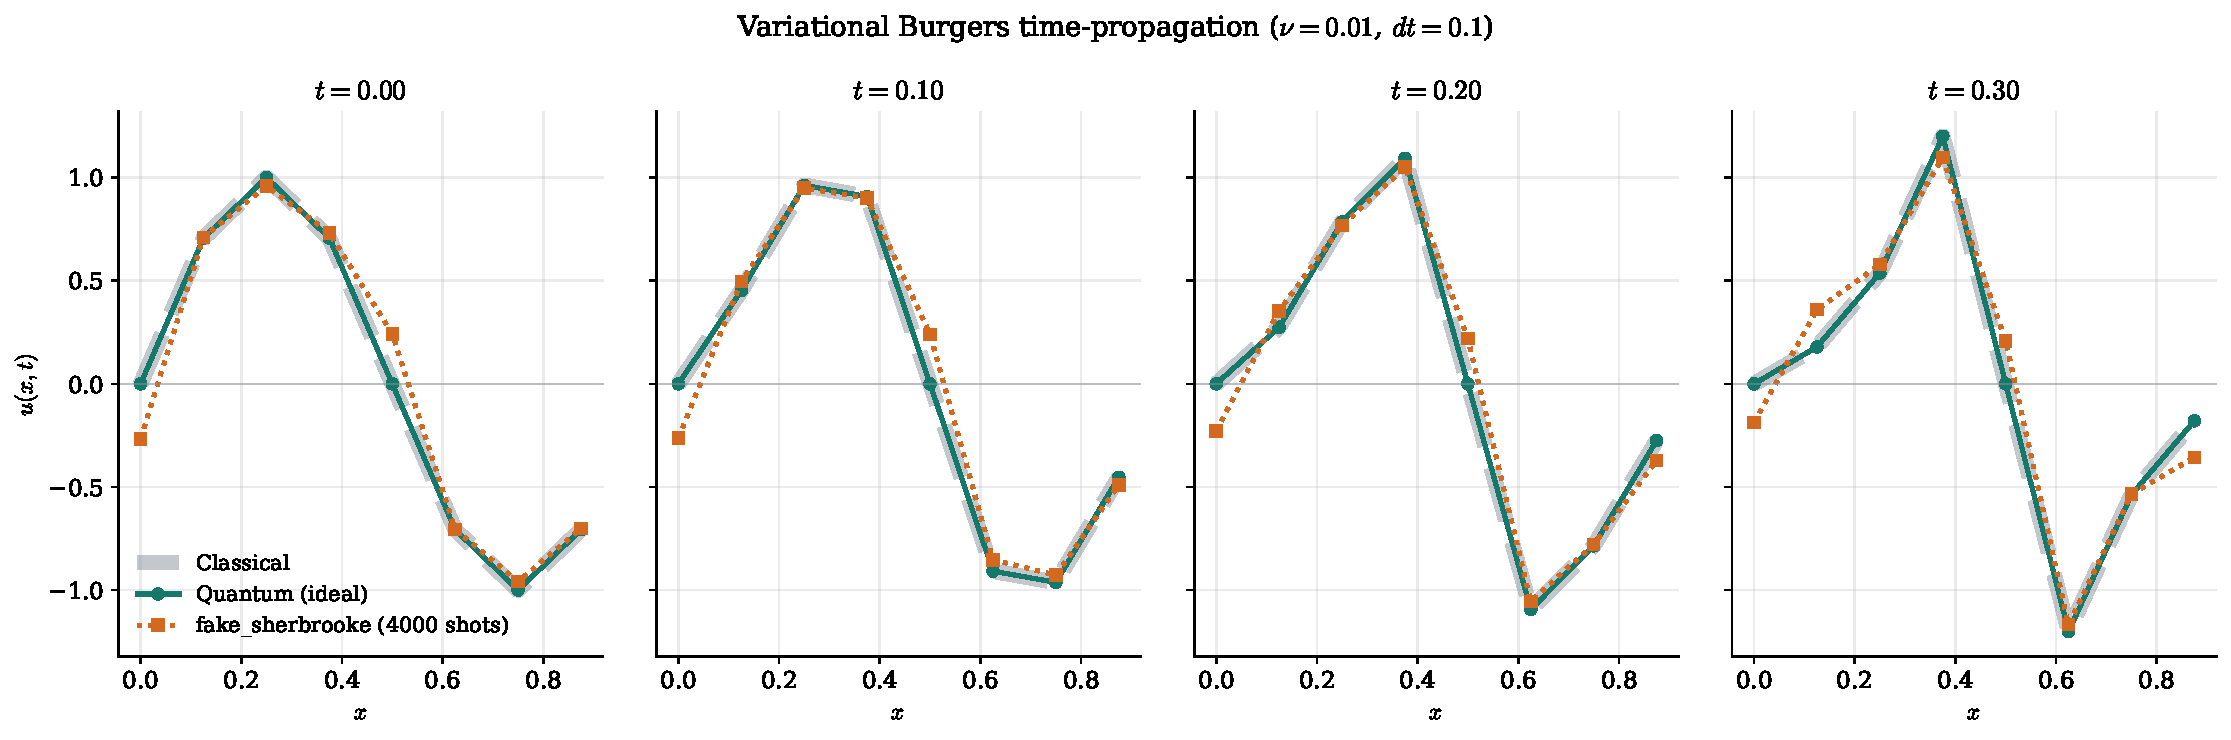
\includegraphics[width=\textwidth]{figures/fig_burgers_variational.pdf}
\caption{Burgers propagation via Route~2: classical (dashed) versus ideal quantum (solid, matching to
$\sim10^{-6}$) versus noisy hardware readout (dotted). Viscosity here is ten times smaller than in
Fig.~\ref{fig:carleman-burgers}, so advective steepening is far more visible before diffusion catches
up, while the maximum principle of Sec.~\ref{sec:intro} still caps $\norm{u(t)}_\infty$.}
\label{fig:burgers-var}
\end{figure*}

\begin{figure*}[t]
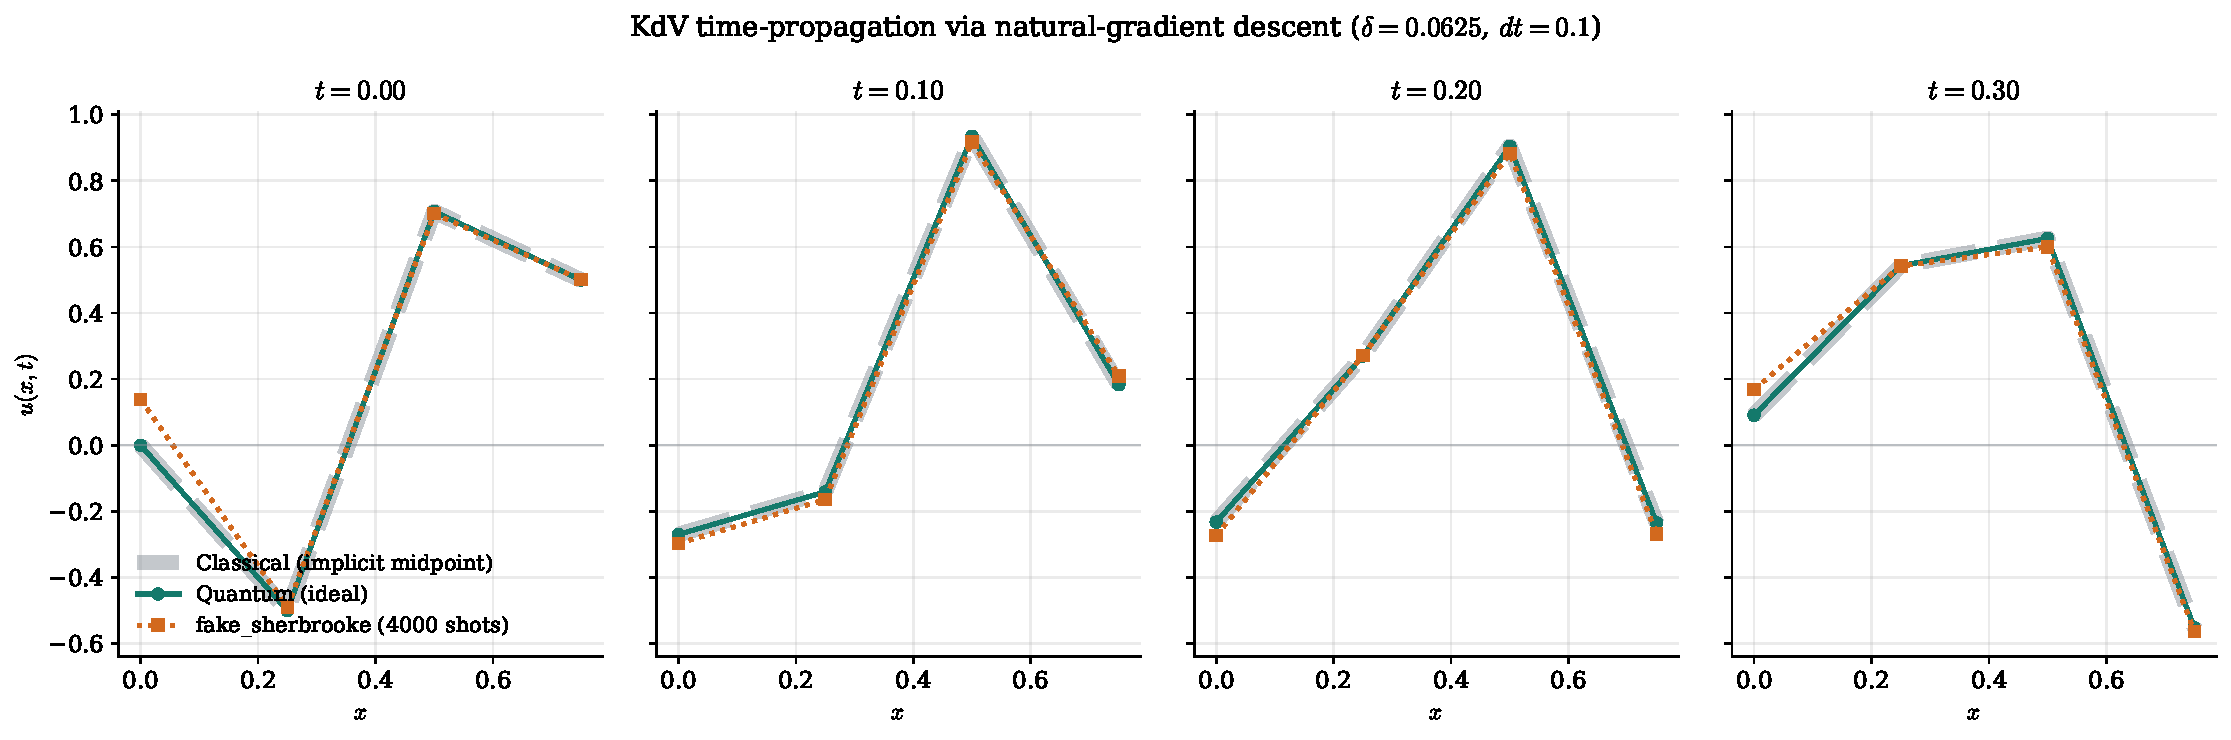
\includegraphics[width=\textwidth]{figures/fig_kdv_variational.pdf}
\caption{KdV propagation via Route~2, with the implicit-midpoint target of Sec.~\ref{sec:midpoint}.
Dispersion replaces Burgers' diffusion: instead of damping gradients it spreads wavelengths at
different phase velocities, turning would-be steepening into an oscillatory wave train rather than a
shock. That mechanism is conservative, not dissipative, which is why $\norm{u}_2$ is held constant to
$10^{-10}$ classically and $\sim10^{-7}$ by the quantum fit, where it strictly decreases for Burgers.}
\label{fig:kdv-var}
\end{figure*}

\subsection{Measured scaling}
\label{sec:varscaling}

We measured how Route~2's resources grow by building and transpiling the actual circuits at
$n=2,\dots,6$ ($n_x=4,\dots,64$) against the \texttt{FakeSherbrooke} calibration snapshot at
optimization level~3, rather than evaluating a closed-form asymptotic alone. Every quantity is
polynomial in $n$ and therefore \emph{polylogarithmic} in grid size: the parameter count is exactly
$P=n(n+1)=\Theta(\log^2n_x)$ at every $n$ tested, transpiled gate counts and depths fit power laws
with exponents in $[1.2,2.6]$, and qubit counts are exactly $\Oh(n)=\Oh(\log n_x)$ --- $n$ for the
identity/linear circuit, $2n$ for the nonlinear one, $n+1$ for the metric.

%=======================================================================
\section{Route 3: analog realization in a degenerate cavity laser}
\label{sec:analog}
%=======================================================================

The third route declines the digital circuit altogether. If a physical system's equations of motion
\emph{are} the target PDE, no embedding is required and no gate count is paid; what is paid instead is
generality, since the platform solves the equation it happens to implement.

\subsection{Platform}

A digital degenerate cavity laser (DDCL) is a self-imaging $4f$ resonator supporting a large number of
transverse laser modes. An aperture mask in a near-field plane defines an array of spatially separated
laser sites, while an intracavity spatial light modulator in the Fourier plane programs the coupling
between them. The nearest-neighbor coupling is complex and programmable in phase,
\begin{equation}
\kappa=Ke^{i\varphi},
\end{equation}
with $K$ the coupling strength and $\varphi$ the coupling phase. Figure~\ref{fig:ddcl} shows the
near-field laser array and the far-field intensity distribution that reports the array's collective
coherence.

\begin{figure}[t]
\centering
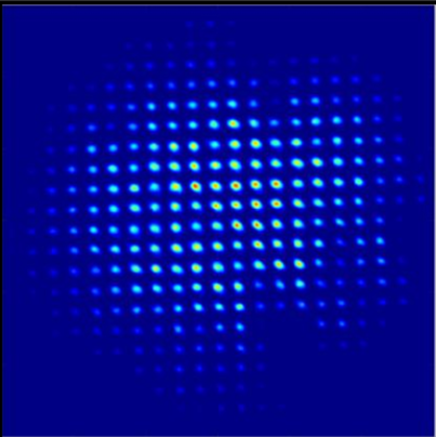
\includegraphics[width=0.44\columnwidth]{figures/ddcl_1.png}\hfill
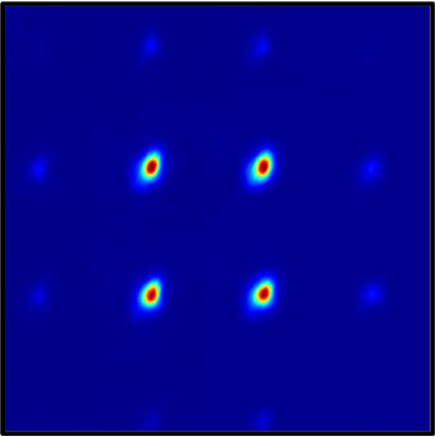
\includegraphics[width=0.44\columnwidth]{figures/ddcl_2.png}
\caption{The analog platform. Left: near-field plane, resolving the individual laser sites of the
programmable array. Right: far-field intensity distribution, which reflects the collective coherence
of the coupled array. Images reproduced from the platform description of Ref.~\cite{DDCL2026}.}
\label{fig:ddcl}
\end{figure}

\subsection{From laser rate equations to Burgers}

The coupled-laser dynamics obey the rate equations
\begin{equation}
\dot E_m=\frac{1}{\tau_c}\Big[(G_m-\alpha_m)E_m+\sum_n\kappa_{mn}E_n\Big],
\end{equation}
together with the gain equation for $G_m$. Writing $E_m=A_me^{-i\theta_m}$, the phase dynamics for
complex nearest-neighbor coupling contains
\begin{equation}
\dot\theta_m=\Omega_m+\frac{K}{\tau_c}\sum_{s=\pm1}\frac{A_{m+s}}{A_m}\sin(\theta_{m+s}-\theta_m-\varphi).
\end{equation}
In the phase-only regime --- approximately equal amplitudes $A_m\simeq A_0$ and identical natural
frequencies --- and after removing the common global rotation, this reduces to the nearest-neighbor
Sakaguchi--Kuramoto model
\begin{equation}
\dot\theta_m=K_{\rm eff}\sum_{s=\pm1}\sin(\theta_{m+s}-\theta_m-\varphi),
\quad K_{\rm eff}=K/\tau_c .
\end{equation}
Introducing $x=ma$ with $a$ the site spacing, taking $\theta_m(t)\to\theta(x,t)$, and expanding for
small nearest-neighbor phase differences gives
\begin{equation}
\theta_t=K_{\rm eff}a^2\cos\varphi\;\theta_{xx}+K_{\rm eff}a^2\sin\varphi\;(\theta_x)^2 .
\end{equation}
Defining the phase-gradient field $u=-2K_{\rm eff}a^2\sin\varphi\;\theta_x$ yields exactly the
one-dimensional viscous Burgers equation,
\begin{equation}
u_t+u\,u_x=\nu_{\rm eff}u_{xx},\qquad \nu_{\rm eff}=K_{\rm eff}a^2\cos\varphi .
\label{eq:ddcl-burgers}
\end{equation}

The physical content of Eq.~\eqref{eq:ddcl-burgers} is worth stating plainly: the optical phase
gradient plays the role of the Burgers field, and the two halves of the complex coupling split the two
halves of the equation between them. The dissipative component $\cos\varphi$ produces the effective
viscosity; the reactive component $\sin\varphi$ produces the advection. Tuning one experimental
parameter therefore tunes the effective Reynolds number continuously --- the same quantity that,
in Sec.~\ref{sec:carleman-conv}, was the binding constraint on Route~1.

\subsection{What the platform delivers, and what it does not}

For a stationary state $u_t=0$, Eq.~\eqref{eq:ddcl-burgers} integrates once to
$u_x+\tan\varphi\,u^2=C$, whose bounded solution is the hyperbolic front
\begin{equation}
u(x)=u_0\tanh\!\Big(\frac{x-x_0}{\ell}\Big),
\end{equation}
with $\ell$ the characteristic front width and $x_0$ fixed by the boundary conditions. Under open
boundary conditions, the experimentally reconstructed stationary phase profile therefore gives direct
access to the corresponding stationary Burgers solution. Table~\ref{tab:ddcl} lists the full
correspondence.

\begin{table}[t]
\caption{Correspondence between the Burgers model and the DDCL platform~\cite{DDCL2026}.}
\label{tab:ddcl}
\begin{ruledtabular}
\begin{tabular}{ll}
Burgers quantity & Experimental realization \\
\hline
$x$ & laser-site position \\
$\theta(x,t)$ & optical phase field \\
$u(x,t)$ & phase-gradient field \\
$K_{\rm eff}$ & coupling strength \\
$\varphi$ & phase of the complex coupling \\
$a$ & spacing between neighboring sites \\
$\nu_{\rm eff}=K_{\rm eff}a^2\cos\varphi$ & effective viscosity \\
\end{tabular}
\end{ruledtabular}
\end{table}

Three limitations should be stated as clearly as the mapping. The correspondence is an effective
phase-only description of the full rate equations, and requires approximately equal amplitudes,
identical natural frequencies, small nearest-neighbor phase differences, and a long-wavelength
continuum limit; outside those conditions the array is not solving Burgers. The accessible observable
demonstrated here is the \emph{stationary} profile, not a time-resolved trajectory, so the analog
route as presented is not yet a like-for-like replacement for the digital routes' propagation results
of Figs.~\ref{fig:carleman-burgers} and~\ref{fig:burgers-var}. And the platform is not programmable
across equations: it realizes Burgers, not KdV, and there is no analog of the truncation-order or
block-encoding knobs that make Routes~1 and~2 general-purpose. What it does supply is an independent,
non-quantum physical realization of the same equation, and evidence that Burgers dynamics are
physically generic rather than an arbitrary benchmark.

%=======================================================================
\section{The three routes compared}
\label{sec:comparison}
%=======================================================================

Table~\ref{tab:comparison} places the three routes side by side. The comparison is not a ranking:
they answer different questions, and the useful content is in \emph{where} each one's cost sits.

\begin{table*}[t]
\caption{The three routes compared, at the problem sizes actually reached in this work.
``Measured'' quantities were built, transpiled, and run; ``projected'' quantities were derived and
calibrated against published gate-level data. Classical reference: pseudo-spectral solve of the same
instance.}
\label{tab:comparison}
\begin{ruledtabular}
\begin{tabular}{lccc}
 & Route 1: Carleman--QSVT & Route 2: variational & Route 3: DDCL analog \\
\hline
Linear embedding required & yes, dimension $\sum_j n_x^j$ & no & no \\
Nonlinearity handled by & the embedding & classical optimizer & the physical medium \\
Qubits (measured) & 6--14 & 2--6 & --- \\
Gates per solve (measured) & $2.6\times10^{6}$--$1.7\times10^{9}$ & 29--351 & --- \\
Scaling in grid size & $\Oh(n_x^4)$ dense encoding & $\Oh(\mathrm{poly}\log n_x)$ & fixed by array size \\
Asymptotic depth (projected) & $\Ot(\kappa_V T\NC^3\Rey^{-1}\epsilon^{-1})$ & not derived & --- \\
Convergence guarantee & yes, but only $\Rey<\pi/2$ & none (nonconvex) & effective-model validity \\
Runs on present hardware & no & yes & yes (is hardware) \\
Accuracy achieved & numerical precision vs.\ classical & $2\times10^{-8}$--$4\times10^{-6}$ ideal & stationary profile \\
Solves KdV as well & yes & yes & no \\
\end{tabular}
\end{ruledtabular}
\end{table*}

Read across the table, three statements follow.

\paragraph{Route 1 buys memory and nothing else, in one dimension.} Its qubit count is genuinely
exponentially smaller than classical memory, and no part of the analysis erodes that. Everything
else is worse than classical: matched $\epsilon$ scaling with large extra factors, inherently
sequential depth, a state rather than a field as output, and a convergence guarantee confined to
$\Rey<\pi/2$. The worked instance of Table~\ref{tab:worked} makes the gap concrete at nine to ten
orders of magnitude after error correction. A crossover in \emph{work} requires three spatial
dimensions, observable-only readout, and a polynomially bounded $\kappa_V$ --- and the non-normality of
Carleman matrices leaves the last of these open.

\paragraph{Route 2 is cheap because it moved the hard part, not because it removed it.} Its circuits
are shallow and its scaling polylogarithmic, but the nonlinear work reappears as a nonconvex
optimization solved afresh at every timestep with no convergence guarantee, and --- in our
implementation --- one residual $\Oh(2^n)$ classical evaluation whenever the certificate of
Proposition~\ref{prop:cert} fails to apply. We reduced that residual to $\sim55$ calls per timestep
and we can bound when it is needed, but making the residual fraction provably $\Oh(\mathrm{poly}(n))$
rather than empirically small remains open. This is the honest statement of the method's status: a
demonstrated present-day capability with a clearly localized theoretical gap.

\paragraph{Route 3 removes the embedding by giving up programmability.} A medium whose native
dynamics are the target equation pays no gate cost at all, and tunes the very parameter that
obstructs Route~1 by rotating a coupling phase. The price is that it solves one equation, under
conditions that must hold for the effective description to be valid, and delivers what the optics can
be made to report.

Underlying all three, the discretization results of Sec.~\ref{sec:discretization} are what make the
comparison meaningful at all. Without the closure of Proposition~\ref{prop:closure}, a discretized
Burgers solution can violate the maximum principle that defines the problem, and a discretized KdV
solution drifts by $11\%$ in a norm the equation conserves exactly. Without the integrator result of
Sec.~\ref{sec:euler}, a variational propagator inherits a monotone energy injection that no circuit
fidelity can remove. Neither is visible in a gate count.

%=======================================================================
\section{Conclusion}
\label{sec:conclusion}
%=======================================================================

We have costed three routes from the same pair of nonlinear PDEs to a quantum-encoded solution, and
held all three to the same physical standard. The Carleman--QSVT route works --- we built it, and every
quantum result matches its classical counterpart to numerical precision --- but its convergence is
provable only for $\Rey<\pi/2$, its block encoding as usually constructed carries a subnormalization
$\alpha\simeq n_x^{\NC-1}\lambda_{\rm cfl}$ that erases the nominal exponential compression, its
sequential stepping requires a history-state dilation to be viable at all, and its assembled depth
$\Ot(\kappa_V T\NC^3\Rey^{-1}\epsilon^{-1})$ evaluates to $1.3\times10^{12}$ logical two-qubit gates
where a laptop needs $4.4\times10^6$ floating-point operations. The variational route reaches the same
physics with circuits of at most $351$ gates on present-day hardware, at the cost of a nonconvex
optimization with no convergence guarantee. The analog route reaches it with no circuit at all, at the
cost of programmability.

The useful output is the decomposition, not a winner. Of Route~1's five cost drivers, the qubit count
is a clean exponential win; the block encoding and the sequential stepping are engineering problems
with identifiable fixes; the readout is a hard barrier only if the full field is wanted; and exactly
one --- the Carleman convergence radius --- is fundamental within the framework. Two methodological
points generalize beyond this problem. First, state which condition number is meant: $\alpha/\sigma_{\min}$
and $\sigma_{\max}/\sigma_{\min}$ differ by a factor of $3.5$ in the published Burgers instance, and
only the former sets the cost. Second, report the polynomial accuracy alongside $\kappa$ and the
degree, without which published pairs cannot be compared.

Finally, the choice of test problem is not innocent. Burgers is linearizable in closed form by
Cole--Hopf, so a Burgers demonstration establishes that circuits compile and produce the right answer
--- valuable, and how we use it --- but cannot by itself establish that a method handles nonlinearity.
Carrying KdV through every stage is what makes the comparison a test rather than an exhibition.

\begin{acknowledgments}
We thank the organizers of the 2026 Niels Bohr Quantum Summer School Challenge on Quantum Simulation
of Nonlinear Partial Differential Equations, Center for Quantum Mathematics, University of Southern
Denmark.
\end{acknowledgments}

\section*{Data and code availability}
All circuits, classical reference solutions, resource-counting scripts, and the numerical validation
of every formula reported here are available in the accompanying repository. The asymptotic analysis
of Sec.~\ref{sec:cost} is reproduced by three short Python scripts requiring only \texttt{numpy} and
\texttt{scipy}; the circuit results of Secs.~\ref{sec:carleman} and~\ref{sec:variational} are
reproduced by four Qiskit notebooks that run end to end.

\section*{AI disclosure}
The physics, algorithms, and the great majority of the code in this work are the authors' own: the
choice of Carleman linearization and QSVT, the variational natural-gradient formulation, the
discretization, the error-budget analysis, and the fixes described throughout originated with the
authors. Claude (Anthropic) was used interactively, under the authors' direction and review, to help
implement specific pieces of that design, debug issues the authors identified, run numerical
verification, and draft parts of this manuscript's text. All physical claims, discretization choices,
and numerical results were independently verified by the authors against classical reference
calculations rather than accepted on the model's assertion alone; every proof was checked step by
step; every cited reference was checked against its original source before inclusion.

\begin{thebibliography}{99}

\bibitem{Setty2026} A.~Setty, ``A quantum linear systems pathway for solving differential equations,''
J. Phys. A: Math. Theor. \textbf{59}, 185303 (2026).

\bibitem{Setty2025BE} A.~Setty, ``Block encoding of sparse matrices via coherent permutation,''
arXiv:2508.21667 (2025).

\bibitem{Liu2021} J.-P.~Liu, H.~{\O}.~Kolden, H.~K.~Krovi, N.~F.~Loureiro, K.~Trivisa, A.~M.~Childs,
``Efficient quantum algorithm for dissipative nonlinear differential equations,'' Proc. Natl. Acad.
Sci. U.S.A. \textbf{118}, e2026805118 (2021).

\bibitem{Forets2017} M.~Forets and A.~Pouly, ``Explicit error bounds for Carleman linearization,''
arXiv:1711.02552 (2017).

\bibitem{Wu2025} H.-C.~Wu, J.~Wang, X.~Li, ``Quantum algorithms for nonlinear dynamics: revisiting
Carleman linearization with no dissipative conditions,'' SIAM J. Sci. Comput. \textbf{47}, A943
(2025).

\bibitem{GonzalezConde2025} J.~Gonzalez-Conde, D.~Lewis, S.~S.~Bharadwaj, M.~Sanz, ``Quantum Carleman
linearization efficiency in nonlinear fluid dynamics,'' Phys. Rev. Research \textbf{7}, 023254 (2025).

\bibitem{Gilyen2019} A.~Gily{\'e}n, Y.~Su, G.~H.~Low, N.~Wiebe, ``Quantum singular value
transformation and beyond: exponential improvements for quantum matrix arithmetics,'' in
\emph{Proceedings of the 51st Annual ACM SIGACT Symposium on Theory of Computing} (STOC 2019),
pp.~193--204.

\bibitem{McLachlan1964} A.~C.~McLachlan, ``A variational solution of the time-dependent Schr\"odinger
equation,'' Mol. Phys. \textbf{8}, 39 (1964).

\bibitem{Li2017} Y.~Li and S.~C.~Benjamin, ``Efficient variational quantum simulator incorporating
active error minimization,'' Phys. Rev. X \textbf{7}, 021050 (2017).

\bibitem{Yuan2019} X.~Yuan, S.~Endo, Q.~Zhao, Y.~Li, S.~C.~Benjamin, ``Theory of variational quantum
simulation,'' Quantum \textbf{3}, 191 (2019).

\bibitem{Mitarai2018} K.~Mitarai, M.~Negoro, M.~Kitagawa, K.~Fujii, ``Quantum circuit learning,''
Phys. Rev. A \textbf{98}, 032309 (2018).

\bibitem{Schuld2019} M.~Schuld, V.~Bergholm, C.~Gogolin, J.~Izaac, N.~Killoran, ``Evaluating analytic
gradients on quantum hardware,'' Phys. Rev. A \textbf{99}, 032331 (2019).

\bibitem{Costa2025} P.~C.~S.~Costa, P.~Schleich, M.~E.~S.~Morales, D.~W.~Berry, ``Further improving
quantum algorithms for nonlinear differential equations via higher-order methods and rescaling,''
npj Quantum Inf. \textbf{11}, 141 (2025).

\bibitem{Harten1983} A.~Harten, ``High resolution schemes for hyperbolic conservation laws,''
J. Comput. Phys. \textbf{49}, 357 (1983).

\bibitem{Tadmor1987} E.~Tadmor, ``The numerical viscosity of entropy stable schemes for systems of
conservation laws. I,'' Math. Comp. \textbf{49}, 91 (1987).

\bibitem{Shende2006} V.~V.~Shende, S.~S.~Bullock, I.~L.~Markov, ``Synthesis of quantum-logic
circuits,'' IEEE Trans. Comput.-Aided Des. Integr. Circuits Syst. \textbf{25}, 1000 (2006).

\bibitem{Fornberg1988} B.~Fornberg, ``Generation of finite difference formulas on arbitrarily spaced
grids,'' Math. Comp. \textbf{51}, 699 (1988).

\bibitem{LeVeque2007} R.~J.~LeVeque, \emph{Finite Difference Methods for Ordinary and Partial
Differential Equations} (SIAM, Philadelphia, 2007).

\bibitem{DDCL2026} ``Analog simulation of Burgers dynamics in a digital degenerate cavity laser,''
Niels Bohr Quantum Summer School 2026, Center for Quantum Mathematics, University of Southern Denmark.

\end{thebibliography}

\end{document}
